\documentclass[11pt]{article}
% Shared preamble of the project's LaTeX notes: notes/*.tex and the documents in literature/.
% Project macros go at the end. A macro copied from a paper's source goes in the note that
% quotes it, between its \input of this file and \begin{document}.
\usepackage[a4paper,margin=25mm]{geometry}
\usepackage{amsmath,amssymb,mathtools,bm}
\usepackage{graphicx,booktabs,xltabular}
\usepackage{xcolor}
\usepackage{xspace}
\usepackage[numbers,sort&compress]{natbib}
\bibliographystyle{apsrev4-2} % prints the arXiv ID of each entry in refs.bib
\usepackage[colorlinks,allcolors=blue!60!black]{hyperref}
\usepackage[notref,notcite]{showkeys} % prints each \label in the margin, so a pointer by label is found in the PDF
\renewcommand*\showkeyslabelformat[1]{\normalfont\tiny\ttfamily#1}

% Ragged-right X column for tables with prose cells: bridges, the survey's term map.
\newcolumntype{L}{>{\raggedright\arraybackslash}X}

% Project macros, in the notation of CONVENTIONS.md.
\newcommand{\GeV}{\mathrm{GeV}}
\newcommand{\MeV}{\mathrm{MeV}}
\newcommand{\vep}{{\bm p}}
\newcommand{\vek}{{\bm k}}
\newcommand{\veq}{{\bm q}}
\newcommand{\ver}{{\bm r}}
\newcommand{\vex}{{\bm x}}
\newcommand{\veA}{{\bm A}}
\newcommand{\vetau}{{\bm \tau}}
\newcommand{\veL}{{\bm L}}
\newcommand{\veS}{{\bm S}}
\newcommand{\ven}{{\bm n}}
\newcommand{\veep}{{\bm \epsilon}}
\newcommand{\veepst}{{\bm \epsilon}^{\prime*}}
\newcommand{\bbnP}{[\bar{b}b]_1(nP)}
\newcommand{\bbarb}{[\bar{b}b]_1}
\newcommand{\psibb}{\Psi^{(\bar{b}b)}}
\newcommand{\Mbb}{M^{(\bar{b}b)}}
\newcommand{\X}{X(3872)}
\newcommand{\Xb}{X_b}
\newcommand{\VQQ}{V^{(\bar{b}b)}}
\newcommand{\VOME}{V^{\rm (OME)}}
\newcommand{\TOME}{T^{\rm (OME)}}
\newcommand{\BOchiEFT}{BO$\chi$EFT\xspace}
\newcommand{\cyan}[1]{\textcolor{cyan}{#1}}

\newcommand{\file}[1]{\nolinkurl{#1}}
\title{S40: one path rule for every energy region}
\author{}
\date{2026-11-13}
\begin{document}
\maketitle

\noindent Derivations and evidence for S40 (\texttt{st:shape}) of \file{notes/07-continued-lse.tex}. On 2026-11-13 the user adopted the deformed SP method (\file{GLOSSARY.md}) in its sheet-as-a-sign form (Sec.~\ref{sec:sign}): one path per search rectangle, on-shell nodes carrying the sheet's sign. The polygon of R1 is the special case that L3 and L5 treat; it is the base point of the continuation argument on each adjacent strip. Statement numbers are those of note~07.

\paragraph{Notation.} $E$ is measured from $2m_{B^*}$. The channels $\alpha=1,5,6$ are $VV$, $PV$, $PP$, with thresholds $\delta_\alpha=0,-45.23,-90.46$~MeV, reduced masses $\mu_\alpha=2662.38,2651.00,2639.76$~MeV and on-shell momenta $k_\alpha=\sqrt{2\mu_\alpha(E-\delta_\alpha)}$. $F$ is the set of flipped channels, $R(\mathcal C)$ the region between $[0,\Lambda]$ and the path $\mathcal C$, $d_k$ the pole margin (\file{CONVENTIONS.md}), and $E_{3,\beta}=m_\phi+t_\beta$ the three-body thresholds, the lowest $E_{3,1}=47.58$~MeV ($B\bar B\pi$). A graph path is $q=x+ih(x)$ with $h(0)=h(\Lambda)=0$; its slopes are at most $1$ when $|h(x)-h(y)|\le|x-y|$.

\paragraph{Prescription and sheets.} With $G_\alpha=2\mu_\alpha/(q^2-k_\alpha^2)$ (S9) the physical amplitude is $T(E+i0)$: $k_\alpha^2$ gets $+i0$, and the pole near $+k$ sits at $q=k+i0$, just above the real path, which passes below it. On the physical sheet $\operatorname{Im}k_\alpha>0$ in every channel; channel $\alpha$ is flipped where $\operatorname{Im}k_\alpha<0$. The real energy axis above a threshold carries two lips: $E+i0$ of the physical sheet is glued to $E-i0$ of the sheet where that channel is flipped, and there $k_\alpha=k-i0$, the flipped momentum just below the real axis. The pole sits at $k-i0$ on both sheets at $E-i0$; for an integral without on-shell subtraction the sheet is decided by the side on which the path passes it:
\begin{center}
\small
\setlength{\tabcolsep}{4pt}
\begin{tabular}{lllll}
\toprule
energy & pole near $+k$ & path passes & channel $\alpha$ & value\\
\midrule
$E+i0$ & $k+i0$ & below & physical & $T(E+i0)$, outgoing waves\\
$E-i0$ & $k-i0$ & above & physical & other boundary value (incoming)\\
$E-i0$ & $k-i0$ & below & flipped & equal to $T(E+i0)$\\
$\operatorname{Re}E-i\Gamma/2$ & $k_\alpha$, $\operatorname{Im}k_\alpha<0$ & below & flipped & continued $T(E+i0)$\\
\bottomrule
\end{tabular}
\end{center}
A flipped pole is therefore $+k_\alpha$ with $\operatorname{Im}k_\alpha<0$: the $k-i0$ of the third row, carried to complex $E$. Without subtraction the path passes below it, $+k_\alpha\in R(\mathcal C)$ (S27). R2 below evaluates the reference polygon in the limit of an indentation below the pole. For a channel treated by subtraction, the same sheet is selected by the sign of the analytic term instead of the path's placement (Sec.~\ref{sec:sign}).

\section{What S40 has to settle}

S40 builds a three-segment path that keeps every pole $\pm k_\alpha$ at a distance $d_k$, with Gauss--Legendre nodes per segment. Three things go wrong.
\begin{enumerate}
\item Just above each threshold the largest admissible margin vanishes. The newly flipped pole tends to $\sqrt{\mu_\alpha|\operatorname{Im}E|}\,(1-i)$, on the line of slope $1$ through the origin, and a path with slopes at most $1$ cannot pass below the line. The largest margin is that pole's distance to the line, $(\operatorname{Re}k_\alpha-|\operatorname{Im}k_\alpha|)/\sqrt2$: $0.6$, $11.5$ and $34.2$~MeV at $0.05$, $1$ and $3$~MeV above the threshold at $\operatorname{Im}E=-10$~MeV. On App.~D's integral of \cite{Wu:2026wxb}, $0.05$~MeV above the $PV$ threshold, $256$ nodes per segment still leave a relative error of $6.2\times10^{-3}$.
\item On-shell $T$ on that path needs S32's depth window for every flipped channel. The single flat depth, set by the deepest pole, breaks it at the $VV$ threshold from $\Gamma=28$~MeV, where it passes below $k_6-im_\pi$.
\item The pole search of S41 certifies one fixed path per energy rectangle. With the poles kept at $d_k$ from a fixed path, the rectangles must shrink towards each threshold.
\end{enumerate}
What is wanted is one rule, simple, explicit for each energy region, valid wherever it claims to be, with the remaining regions excluded by name.

\section{A reference polygon on an adjacent strip}

Let $\operatorname{Im}E\le0$ and $\operatorname{Re}E\ne\delta_\alpha$, on the sheet attached at $\operatorname{Re}E$, $F=\{\alpha:\delta_\alpha<\operatorname{Re}E\}$ (S27).
\begin{description}
\item[R1, reference path.] For the proof on the adjacent strip, take $\mathcal C(E)$ to be the polygon through the flipped poles in increasing $\operatorname{Re}k$:
\[
0\ \to\ k_{(1)}\ \to\ \dots\ \to\ k_{(|F|)}\ \to\ \Lambda .
\]
For $F=\emptyset$ it is $[0,\Lambda]$.
\item[R2, subtraction.] On this reference polygon the flipped pole $k_\alpha$ is a vertex, and its analytic integral has the value for a path passing just below it. Subtraction does not require this geometry (Sec.~\ref{sec:sign}). With $\Phi(q)=V_{\alpha'\alpha}(p',q)\,T_{\alpha\alpha''}(q,p)$ and $G_\alpha(q)=2\mu_\alpha/(q^2-k_\alpha^2)$ as in S9,
\begin{equation}\label{eq:split}
\int_{\mathcal C}q^2dq\,G_\alpha(q)\,\Phi(q)=2\mu_\alpha\int_{\mathcal C}dq\,\frac{q^2\Phi(q)-k_\alpha^2\Phi(k_\alpha)}{q^2-k_\alpha^2}+2\mu_\alpha k_\alpha^2\,\Phi(k_\alpha)\,I(k_\alpha),
\end{equation}
\begin{equation}\label{eq:I}
I(k)=\int_{\mathcal C\ \text{below}\ k}\frac{dq}{q^2-k^2}=\frac1{2k}\Bigl[\operatorname{Log}\frac{\Lambda-k}{\Lambda+k}+i\pi\Bigr].
\end{equation}
On the nodes this adds one node $q=k_\alpha$ per flipped channel, with weight
\begin{equation}\label{eq:W}
W_\alpha=2\mu_\alpha k_\alpha^2\Bigl[I(k_\alpha)-\sum_j\frac{\omega_j}{q_j^2-k_\alpha^2}\Bigr],
\end{equation}
so that $\mathcal G$ of S9 gains the entry $W_\alpha/2\pi^2$, and $V$ and $T$ gain the row and column at $k_\alpha$. The bracket is the quadrature error of $I(k_\alpha)$ on the nodes; Eq.~\eqref{eq:W} hands it to the on-shell value $\Phi(k_\alpha)$.
\item[R3, kernel.] Principal $s_\pm$ and logarithms at every pair of $\mathcal C\times\mathcal C$, including the vertices (S34, S35); no tracker.
\item[R4, quadrature.] Composite Gauss--Legendre: panel ends at $0$, at every vertex and at $\Lambda$, each segment cut into equal panels no longer than $L_p$, with $n_p$ nodes per panel. $L_p$ and $n_p$ come from the Stage~6 convergence run; start at $L_p=250$~MeV, $n_p=16$.
\item[R5, pole search.] A rectangle has $\operatorname{Im}E<0$ and lies inside one strip: between two consecutive thresholds, or between $\delta_1$ and $E_{3,1}$. The vertices follow $E$; the number of panels of each segment is fixed at the rectangle's centre, with panel ends at fixed fractions of each segment. The discrete $D_{\mathcal C}(E)$ is then meromorphic on the rectangle (L6), and no path is certified per rectangle.
\item[R6, on-shell quantities.] $T_{\alpha\beta}(k_\alpha,k_\beta)$, $\alpha,\beta\in F$, are entries of the same solution; the homotopy $\mathcal H$ of L3 certifies them (L5). The on-shell-point identities \texttt{06:eq:onshellpoint}--\texttt{06:eq:Dflip}, which go back to $[0,\Lambda]$, remain a check only where no singular point of $V(k_F,q)$ has crossed $[0,\Lambda]$ (S32, second condition).
\end{description}

\section{Scenarios}

\begin{center}
\small
\begin{tabular}{>{\raggedright\arraybackslash}p{0.24\textwidth}>{\raggedright\arraybackslash}p{0.11\textwidth}>{\raggedright\arraybackslash}p{0.2\textwidth}>{\raggedright\arraybackslash}p{0.32\textwidth}}
\toprule
region & sheet, $F$ & example path & treatment, status\\
\midrule
$\operatorname{Im}E=0$, $\operatorname{Re}E<-90.46$: bound states & $(+,+,+)$, $\emptyset$ & $[0,\Lambda]$ & R3, R4; poles on the negative imaginary axis. In scope, as for $1^{++}$.\\
$-90.46<\operatorname{Re}E<-45.23$, $-10\le\operatorname{Im}E<0$ & $(-,+,+)$, $\{6\}$ & $0\to k_6\to\Lambda$ & R2 at $k_6$. In scope.\\
$-45.23<\operatorname{Re}E<0$, $-10\le\operatorname{Im}E<0$: the $X_{b2}$ region & $(-,-,+)$, $\{5,6\}$ & $0\to k_5\to k_6\to\Lambda$ & R2 at $k_5$, $k_6$. In scope.\\
the same strips, $-50\le\operatorname{Im}E<-10$ & as above & as above & as above. Widening to $\Gamma\le100$~MeV.\\
$0<\operatorname{Re}E<37.58$ & $(-,-,-)$, $\{1,5,6\}$ & $0\to k_1\to k_5\to k_6\to\Lambda$ & R2 at all three; S35 without the $H^2$ term (L4) where $\operatorname{Re}E>47.58-H^2/m_B$. Widening to $(-,-,-)$.\\
$37.58\le\operatorname{Re}E<47.58$ & $(-,-,-)$ & as above & and panels graded geometrically towards $q=0$, where three-body points come within $17$--$53$~MeV. Widening, with its own convergence run.\\
$\operatorname{Im}E=0$ above a threshold: $T(E+i0)$ & limit of the adjacent sheet & $[0,\Lambda]$ & R2 at the real $k_F$, the limit $\operatorname{Im}E\to0^-$. The real $k_F$ need not be a panel break. Checks and the speed plot.\\
$\operatorname{Re}E=\delta_\alpha$ & -- & -- & a branch point of $D$; rectangles end there. Excluded points.\\
$\operatorname{Re}E\ge47.58$ & -- & -- & the three-body cut opens; S35 fails. Outside (S2).\\
virtual states: a channel flipped below its threshold, e.g.\ $(-,-,-)$ below $\delta_1$ & not adjacent & -- & the flipped pole lies below the slope-1 line, so the path needs a leg steeper than $1$ and L1, L4, L5 do not apply. On the real axis the vertex $k_1=-i\kappa_1$ meets the $VV$ pion cut of the amplitude itself at $\kappa_1=m_\pi/2=69.02$~MeV ($E_B=0.89$~MeV), at $52.13$~MeV ($0.51$~MeV) on one common path (note~06, Sec.~\texttt{lhc}); a deeper virtual state is reported with a side. Stage~8.\\
hidden poles: a channel unflipped above its threshold & not adjacent & -- & the polygon keeps the pole outside $R(\mathcal C)$ in some cases ($VV$ on $(-,-,+)$ above $\delta_1$), not in others ($PP$ on $(+,-,+)$ between $\delta_5$ and $\delta_1$), which need a vertex passed above; the sheet is reached around a threshold, which L3 and L5 do not cover. Stage~8.\\
couplings to unflipped channels & -- & -- & on-shell $T$ at an unflipped $k_\alpha$ is no entry of the solution (R6); beyond that channel's on-shell pion branch point, e.g.\ the $B^*\bar B^*$ coupling of a $(-,-,+)$ pole with $E_B>0.89$~MeV, it is reported with a side (note~06). Stage~8.\\
\bottomrule
\end{tabular}
\end{center}

The rows outside the rule are drawn in Fig.~\ref{fig:notcovered} (\file{not_covered.py}).
\begin{figure}[ht]
\centering
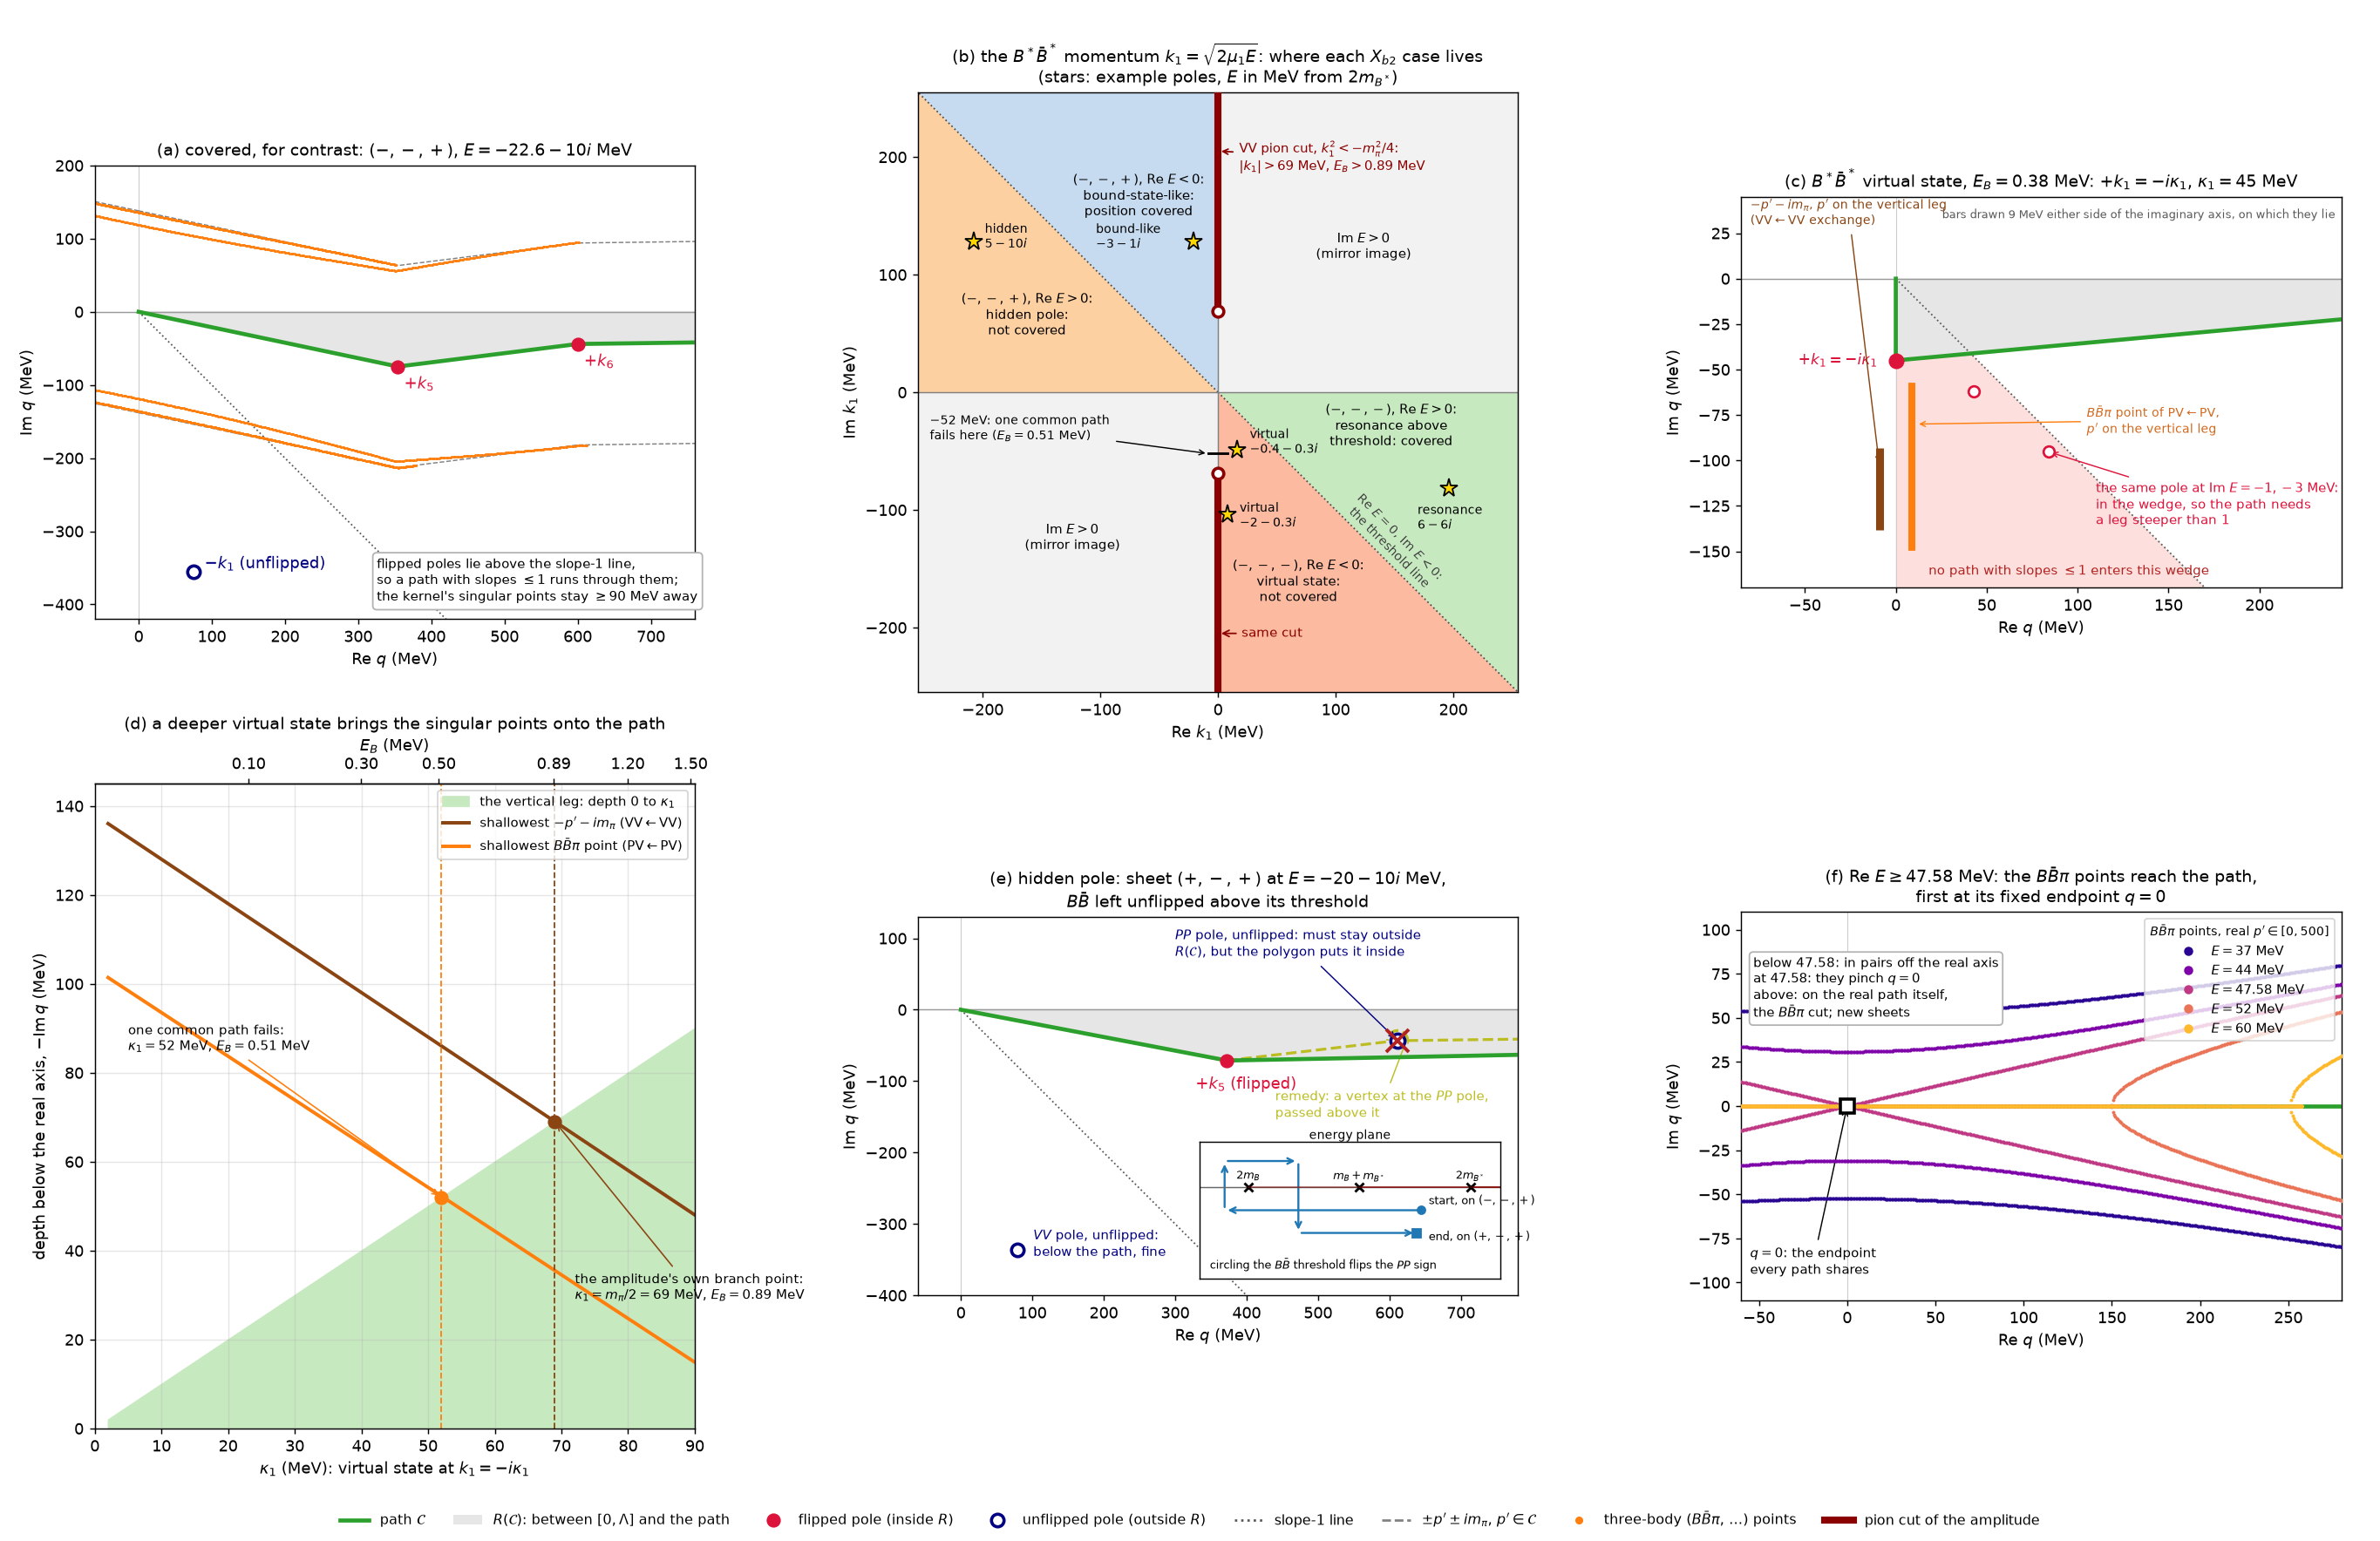
\includegraphics[width=\textwidth]{not_covered.png}
\caption{The cases the rule does not cover, from note~07's formulas, drawn for the idea. (a) A covered case, for contrast. (b) The $B^*\bar B^*$ momentum $k_1$: the wedge of each $X_{b2}$ scenario, and the $VV$ pion cut $k_1^2<-m_\pi^2/4$ of the on-shell amplitude. (c) A virtual state, $E_B=0.38$~MeV: the pole lies in the wedge no path with slopes at most $1$ enters; the vertical leg brings $-p'-im_\pi$ and the $B\bar B\pi$ point of $PV\leftarrow PV$ along. (d) Their shallowest depth against $\kappa_1$: they reach the leg at $\kappa_1=52$ and $69$~MeV. (e) A hidden pole on $(+,-,+)$: the polygon puts the unflipped $PP$ pole inside $R(\mathcal C)$; inset, the energy path to that sheet. (f) The $\beta=1$ three-body points for real $p'$ at real $E$: they pinch the endpoint $q=0$ at $E_{3,1}=47.58$~MeV and lie on the real path above it.}
\label{fig:notcovered}
\end{figure}

\section{Continuation on the reference polygon}

\paragraph{L1: the path exists, with slopes at most 1.} For $\alpha\in F$ write $E-\delta_\alpha=\varepsilon_\alpha-i\Gamma/2$, $\varepsilon_\alpha>0$, $\Gamma>0$. The flipped pole is the principal root, so $\arg k_\alpha=\tfrac12\arg(E-\delta_\alpha)\in(-\pi/4,0)$: with $x_\alpha=\operatorname{Re}k_\alpha$ and $y_\alpha=|\operatorname{Im}k_\alpha|$, $x_\alpha>y_\alpha>0$. From $k_\alpha^2=2\mu_\alpha(E-\delta_\alpha)$,
\[
x_\alpha^2-y_\alpha^2=2\mu_\alpha\varepsilon_\alpha,\qquad x_\alpha y_\alpha=\mu_\alpha\Gamma/2 .
\]
So the flipped poles lie between $[0,\infty)$ and the slope-1 line, on the curve $xy=\mu\Gamma/2$; the one just flipped has the smallest $x$ and the largest $y$. The first segment has slope $y_{(1)}/x_{(1)}<1$. Between consecutive vertices, $x_{(i)}<x_{(i+1)}$, $y=\mu\Gamma/2x$ gives
\[
\frac{y_{(i)}-y_{(i+1)}}{x_{(i+1)}-x_{(i)}}=\frac{y_{(i)}}{x_{(i+1)}}+\frac{\Gamma}{2}\,\frac{\mu_{(i)}-\mu_{(i+1)}}{x_{(i+1)}(x_{(i+1)}-x_{(i)})} .
\]
The first term is below $x_{(i)}/x_{(i+1)}=1-(x_{(i+1)}-x_{(i)})/x_{(i+1)}$, because $y_{(i)}<x_{(i)}$. The second vanishes for equal reduced masses and is positive here, $\mu_{(i)}-\mu_{(i+1)}\approx11$~MeV; the sum stays below $1$ whenever $(\Gamma/2)(\mu_{(i)}-\mu_{(i+1)})<(x_{(i+1)}-x_{(i)})^2$. The gaps exceed $140$~MeV for $\Gamma\le100$~MeV and $\operatorname{Re}E<E_{3,1}$, so this holds by a factor above $30$; the second term itself is below $10^{-3}$ for $\Gamma\le20$~MeV and below $6\times10^{-3}$ for $\Gamma\le100$~MeV. The last segment rises to $\Lambda$ with slope $y_{(|F|)}/(\Lambda-x_{(|F|)})<1$. Hence $\mathcal C(E)$ is a graph path with slopes at most $1$, and $|h(x)|\le x$ because $h(0)=0$. The scan of Sec.~\ref{sec:evidence} finds largest slopes $0.995$ in the search domain and $0.999$ up to $\Gamma=100$~MeV.

\paragraph{L2: placement.} Flipped poles lie on $\mathcal C$, counted as inside $R(\mathcal C)$ by R2 (L3). An unflipped channel, $\delta_\alpha>\operatorname{Re}E$, has $\arg(E-\delta_\alpha)\in(-\pi,-\pi/2)$, so the fourth-quadrant pole of S27 has argument in $(-\pi/2,-\pi/4)$: strictly below the slope-1 line. $\mathcal C$ lies on or above that line ($|h(x)|\le x$), so the pole is outside $R(\mathcal C)$ and off $\mathcal C$, as S27 requires. The placement needs no check.

\paragraph{L3: the homotopy, (P), and the vertex.} The rule comes with its own homotopy $\mathcal H$. (i)~From $E_0=\operatorname{Re}E_1+i\eta$, with $\eta>0$ small, down to $\operatorname{Re}E_1+i0$ on $[0,\Lambda]$: the poles stay in the open first and third quadrants, and at $\operatorname{Re}E_1+i0$ the flipped ones are real, in $(0,\Lambda)$. (ii)~$E_\lambda=\operatorname{Re}E_1+i\lambda\operatorname{Im}E_1$, $0\le\lambda\le1$, with $\mathcal C_\lambda=\mathcal C(E_\lambda)$: every flipped pole is a vertex at every $\lambda$, passed just below (indented by a fixed small $\epsilon$), and every unflipped pole lies below the slope-1 line (L2). So (P) holds along all of $\mathcal H$. With each segment mapped onto a fixed parameter interval, the breakpoints do not move in $t$, as S25 requires.

Note~07's S30 also certifies $D$, with $\mathcal C=\mathcal C(E_1)$ fixed: stage (a) scales the depth at $E_1^*$, $\operatorname{Im}E_1^*>0$, where (P) holds by S29; stage (b) lowers $E=\operatorname{Re}E_1+iy$. An unflipped pole stays in the third quadrant for $y>0$, on the negative imaginary axis at $y=0$, and below the slope-1 line for $y<0$: never on $\mathcal C$. A flipped pole keeps $x^2-y_k^2=c_\alpha\equiv2\mu_\alpha(\operatorname{Re}E_1-\delta_\alpha)>0$, since $\operatorname{Re}E$ is fixed: it runs on the right branch of this hyperbola from the first quadrant, through the real point $\sqrt{c_\alpha}\in(0,\Lambda)$, to its vertex. At a height $s$, $\operatorname{Im}k_\alpha(E_1)<s<0$, it sits at $x=\sqrt{c_\alpha+s^2}$. The path crosses that height twice. On the first segment the crossing is at $x_L=|s|\,x_{(1)}/y_{(1)}$, and $x_L^2=s^2c_{(1)}/y_{(1)}^2+s^2<c_{(1)}+s^2\le c_\alpha+s^2$, because $|s|<y_{(1)}$ and $c_\alpha\ge c_{(1)}$ ($\varepsilon_\alpha\ge\varepsilon_{(1)}+45.23$~MeV, which the spread of the $\mu_\alpha$, at most $23$~MeV, cannot undo). After the vertex the path rises, so the other crossing is at $x_R\ge x_\alpha=\sqrt{c_\alpha+y_\alpha^2}>\sqrt{c_\alpha+s^2}$. So the pole lies inside $R(\mathcal C)$ at every height above its vertex and meets $\mathcal C$ only at the end, at its own vertex, from inside. The two homotopies share the energy path, so they give the same $D$ (S31). For on-shell quantities S30 is not enough (L5).

At the end, indent $\mathcal C$ below each vertex by $\epsilon$. The indented path is admissible for small $\epsilon$; by S25 its $D$ does not depend on $\epsilon$. In each Fredholm term, split as in Eq.~\eqref{eq:split}, the subtracted integrand is analytic near $k_\alpha$, and $\int dq/(q^2-k_\alpha^2)$ along the indented path equals Eq.~\eqref{eq:I} for every $\epsilon$ by Cauchy's theorem. So R2 gives the continued $D$, and Eq.~\eqref{eq:W} is its Nystr\"om form (S26). Eq.~\eqref{eq:I} times $\mu_\alpha k_\alpha^2/\pi^2$, plus $\mu_\alpha\Lambda/\pi^2$, is the rank-one loop of the Stage~3 check (\file{checks/_rank_one.jl}).

\paragraph{L4: (K).} S34: no exchanged-meson branch point lies on a graph path, and $s_\pm$ is principal on $\mathcal C\times\mathcal C$. S35: on a path with slopes at most $1$ and depth $H$, $\operatorname{Re}Z^{(\beta)}_\pm\ge E_{3,\beta}-(h_\beta+a_\beta)H^2-\operatorname{Re}E$. Here $H=y_{(1)}$, and $y_{(1)}^2<x_{(1)}y_{(1)}=\mu_{(1)}|\operatorname{Im}E|$, so $H<\sqrt{\mu_1|\operatorname{Im}E|}$: $163.2$~MeV for $\Gamma\le20$~MeV and $364.9$~MeV for $\Gamma\le100$~MeV. S35 as printed then certifies (K) for $\operatorname{Re}E<42.5$~MeV and $<22.4$~MeV respectively: the first four rows of the table entirely. Without the $H^2$ term the bound is stronger and its proof shorter: $|h(x)|\le x$ gives $\operatorname{Re}p'^2=x^2-h(x)^2\ge0$, likewise $\operatorname{Re}q^2\ge0$, so
\[
\operatorname{Re}Z^{(\beta)}_\pm\ \ge\ E_{3,\beta}-\operatorname{Re}E\ >\ 0\qquad\text{for }\operatorname{Re}E<E_{3,1}.
\]
This covers the $(-,-,-)$ rows. Stage (ii) of $\mathcal H$ (L3) and both stages of S30 keep $\operatorname{Re}E$ fixed, so the bound holds along either homotopy. For $\eta$ exchange $E_{3,\beta}\ge457$~MeV.

\paragraph{L5: the on-shell node.} The on-shell node brings in the half-off-shell kernel $V(k_F,q;E)$, its column $V(p',k_F;E)$, and the diagonal $V(k_F,k_F;E)$. By S4 and S16 their singular points are the zeros of $w_\pm$ (exchanged-meson, $q=\pm k_F\pm im_\phi$) and of $Z^{(\beta)}_\pm$ (three-body), for the orderings of the blocks with an $F$ leg: $\beta=2,3$ for $F=VV$, $1,2,4$ for $PV$, $4$ for $PP$ (S3). By time reversal, $V_{\alpha'\alpha}(p',q)=V_{\alpha\alpha'}(q,p')$ (the Stage~5 time-reversal check of S43), the column is a row with $h_\beta\leftrightarrow a_\beta$, so rows suffice.

\emph{Statement.} Along $\mathcal H$, for every flipped $F$, block with an $F$ leg, ordering $\beta$, meson $\phi$, every $\lambda$ and every $q\in\mathcal C_\lambda$:
(a)~$\operatorname{Re}w_\pm(k_F,q)\ge m_\phi^2$, so $s_\pm$ is principal and $\operatorname{Re}s_\pm\ge m_\phi$;
(b)~$\operatorname{Re}Z^{(\beta)}_\pm(k_F,q;E_\lambda)\ge E_{3,\beta}-(h_\beta+a_\beta)H_\lambda^2-\operatorname{Re}E_1>0$, with $H_\lambda$ the depth of $\mathcal C_\lambda$, and $\ge E_{3,\beta}-\operatorname{Re}E_1$ without the $H^2$ term;
(c)~at the node itself,
\begin{equation}\label{eq:diag}
Z^{(\beta)}_-(k_F,k_F;E)=E_{3,\beta}-\delta_F+c_{F\beta}\,(E-\delta_F),\qquad c_{F\beta}=2\mu_F(h_\beta+a_\beta)-1,
\end{equation}
with $c_{F\beta}=0$, $+0.0043$ ($VV$; $\beta=2,3$), $+0.0043$, $-0.0043$, $0$ ($PV$; $\beta=1,2,4$) and $-0.0043$ ($PP$; $\beta=4$). For the pion $E_{3,\beta}-\delta_F$ is $138.04$, $92.81$ ($VV$), $92.81$, $183.27$, $138.04$ ($PV$) and $183.27$~MeV ($PP$): the gap between the three-body threshold and the on-shell channel's own threshold;
(d)~hence $V(k_F,\cdot\,)$ and $V(\cdot\,,k_F)$ are analytic on a neighbourhood of $\mathcal C_\lambda$ at every $\lambda$; no singular point of the on-shell kernel meets the path, and S32's first condition holds along $\mathcal H$.

\emph{Proof.} In stage (ii), $k_F=x_F+ih_\lambda(x_F)$ is a point of the graph path $\mathcal C_\lambda$; let $q=y+ih_\lambda(y)$. Slopes at most $1$ (L1) give $|\operatorname{Im}(k_F-q)|=|h_\lambda(x_F)-h_\lambda(y)|\le|x_F-y|=|\operatorname{Re}(k_F-q)|$, and $|h_\lambda(x)|\le x$ gives $|\operatorname{Im}(k_F+q)|\le x_F+y=\operatorname{Re}(k_F+q)$. So $\operatorname{Re}(k_F\pm q)^2\ge0$ and $\operatorname{Re}w_\pm\ge m_\phi^2$; for the principal root $(\operatorname{Re}s)^2=(|w|+\operatorname{Re}w)/2\ge\operatorname{Re}w$, which is (a). With $\operatorname{Re}k_F^2=x_F^2-h_\lambda(x_F)^2\ge0$ (or $\ge-H_\lambda^2$) and likewise for $q$, $\operatorname{Re}Z=\operatorname{Re}s+t_\beta+h_\beta\operatorname{Re}k_F^2+a_\beta\operatorname{Re}q^2-\operatorname{Re}E_1$ gives (b), with $H_\lambda<\sqrt{\mu_1|\operatorname{Im}E_1|}$ as in L4. This is S35 with $p'=k_F$: nothing beyond S35 is used, because the on-shell node is a point of the path. (c): at $q=k_F$, $s_-=m_\phi$ and $k_F^2=2\mu_F(E-\delta_F)$. (d): (a) and (b) keep $w_\pm$ off $(-\infty,0]$ and $Z_\pm$ off $0$ uniformly on the compact $\mathcal C_\lambda$. In stage (i), $q$ is real and $k_F$ nearly real; $\operatorname{Re}(k_F\pm q)^2\ge-(\operatorname{Im}k_F)^2$ gives $\operatorname{Re}w_\pm\ge m_\phi^2-(\operatorname{Im}k_F)^2>0$ and $\operatorname{Re}Z\ge E_{3,\beta}-\operatorname{Re}E_1-O((\operatorname{Im}k_F)^2/m_\phi)>0$ for small $\eta$. $\square$

\emph{Why S30's fixed path fails here.} At $E_1^*$ the on-shell momentum is $\overline{k_F(E_1)}$, with $\operatorname{Im}k_F=+y_F$, and its down point $k_F-im_\phi$ sits at height $y_F-m_\phi$, while the fixed path is at depth $y_F$ at $\operatorname{Re}k_F$ (the vertex). For $y_F>m_\phi/2$ the down point starts above the path, inside $R(\mathcal C)$ or, for $y_F>m_\phi$, above the real axis, and it ends below the path: it crosses it during stage (b). For the pion this happens once $|\operatorname{Im}k_F|>69$~MeV, i.e.\ for $\Gamma>2(m_\pi/2)^2/\mu_\alpha=3.6$~MeV next to a threshold, where $|\operatorname{Im}k_F|\simeq\sqrt{\mu_\alpha\Gamma/2}$. $D$ is unaffected, since it has no on-shell node. Along $\mathcal H$ the depth at $\operatorname{Re}k_F$ equals $|\operatorname{Im}k_F|$ at every $\lambda$, the window S32 asks for.

\paragraph{L6: analytic in $E$.} Inside one strip the vertices $k_\alpha(E)$ are analytic in $E$. With the panel counts fixed, every node $q_j(E)=a(E)+t_j[b(E)-a(E)]$ and weight $\omega_j(E)=w_j[b(E)-a(E)]$ is analytic; the kernel on $\mathcal C\times\mathcal C$ is analytic (L4); $I(k)$ is analytic for $k$ in the open fourth quadrant with $|k|<\Lambda$. So the discrete $D_{\mathcal C}(E)$ is meromorphic on the rectangle, with poles only at the bare energies (S11). In the continuum, $D_{\mathcal C(E)}(E)=D_{\mathcal C'}(E)$ for any admissible $\mathcal C'$ near $E$ (S31), which is analytic. At a strip edge the vertex tends to the slope-1 line and $D_{\mathcal C}$ stays continuous; the threshold itself is a branch point.

\section{Evidence so far}\label{sec:evidence}

Plots of the note's formulas, not checks. No linear equation has been solved on $\mathcal C(E)$ yet; the kernel at complex momenta is Stage~5.
\begin{itemize}
\item App.~D's $J(p;m)$ of \cite{Wu:2026wxb}, an on-shell kernel times the propagator, with $p=k_5$ and $m=m_\pi$ (\file{onshell_lhc.py}, Fig.~\ref{fig:routes}). With R2 it equals the exact value to 30 digits for $\Gamma=2$--$40$~MeV, $1$~MeV above the $PV$ threshold. With fixed Gauss--Legendre nodes at $\Gamma=20$~MeV, $0.05$ and $1$~MeV above that threshold, it gives $7.9\times10^{-15}$ and $8.3\times10^{-15}$ at $24$ nodes per segment and $4.9\times10^{-16}$ and $2.6\times10^{-16}$ at $32$; the S40 path at $d_k=d_{k,\max}/2$ with plain nodes gives $6.2\times10^{-3}$ and $6.6\times10^{-11}$ at $256$.
\item On a grid $0.05$--$15$~MeV above each threshold, $\Gamma=1$--$40$~MeV, $\mathcal C(E)$ sweeps no singular point of $V(k_F,q)$; the nearest is $92$~MeV away (\file{onshell_lhc_where.png}).
\item The on-shell node along $\mathcal H$ (\file{onshell_topt.py}, Fig.~\ref{fig:topt}): $114$ energies, $42$ on $(-,+,+)$, $42$ on $(-,-,+)$ and $30$ on $(-,-,-)$, at $0.05$, $1$ and $5$~MeV from each threshold and mid-strip, $\Gamma=2$--$100$~MeV, $21$ steps of $\lambda$ each, $\pi$ and $\eta$, every $\beta$. The smallest distance from $\mathcal C_\lambda$ to a singular point of $V(k_F,q)$ is $97.7$, $92.1$ and $73.3$~MeV on the three sheets; the smallest $\operatorname{Re}Z$ with $p'=k_F$, $q\in\mathcal C_\lambda$ is $137.5$, $92.4$ and $47.4$~MeV; the smallest $\operatorname{Re}w_\pm/m_\phi^2$ is $1.000$; no point is on the wrong side at any $\lambda$. The diagonal stays at or above $138.0$, $92.8$ and $47.6$~MeV, the last for $\beta=1$, which does not occur with an outgoing $VV$ leg. On the same grid S30's fixed path puts a down point on the wrong side at $79$ of the $114$ energies, all with $\Gamma\ge10$~MeV.
\item The same file, an integral with one on-shell TOPT leg: $J=\int dq\,q^2G_F(q)\,M_0(\nu_\beta)(k_F,q)$, with $M_0=[\operatorname{Log}Z_+-\operatorname{Log}Z_-]/2k_Fq$ the $m=0$ moment of S3, at $30$ energies ($\Gamma=2$, $20$, $60$~MeV; $0.05$ and $1$~MeV above each threshold, $1$~MeV below $\delta_1$, mid-strip, and $20$~MeV on $(-,-,-)$), every flipped $F$ and every $\beta$ of its blocks, $111$ cases. Route~3 (R2 on $\mathcal C(E)$, $24$ nodes per $250$~MeV panel, double precision) against route~1 (the S40 path at $d_{k,\max}/2$, no subtraction, adaptive quadrature at $20$ digits): $104$ comparable cases, largest relative difference $1.3\times10^{-15}$. Against route~2 ($[0,\Lambda]$ plus the pole term $2\pi i\mu_Fk_FM_0(k_F,k_F)$, no cut terms): $69$ cases with no up point crossed, largest difference $1.2\times10^{-15}$. Where an up point has crossed $[0,\Lambda]$ ($42$ cases, three-body points included), route~2 misses by $6.9\times10^{-4}$ to $0.23$: the cut terms of App.~D. Where an on-shell point lies between the S40 path and $\mathcal C(E)$ ($7$ cases, where the flat depth sweeps a down point), route~1 misses by $6.3\times10^{-5}$ to $5.5\times10^{-2}$: there the S40 path is the wrong one.
\item Region scan (\file{sp_rule.py}, Fig.~\ref{fig:rule}), with $p'$ sampled on $\mathcal C(E)$, $\pi$ and $\eta$, all orderings. The near-origin entries of the unflipped column come from $|k|\approx52$~MeV, $\Gamma\approx1$~MeV, just below a threshold, where the pole's residue in $q^2G$ is proportional to $k$.
\end{itemize}
\begin{center}
\small
\setlength{\tabcolsep}{4pt}
\begin{tabular}{lrcccc}
\toprule
region & energies & slope & \multicolumn{2}{c}{nearest singular point (MeV)} & nearest unflipped\\
 & & & exchanged & three-body & pole (MeV)\\
\midrule
bound states, $\operatorname{Im}E=0$ & 5 & 0 & 138.0 & 138.0 & 53.4\\
$(-,+,+)$, $\Gamma\le20$ & 44 & 0.995 & 97.9 & 97.8 & 38.1\\
$(-,-,+)$, $\Gamma\le20$ & 44 & 0.995 & 97.9 & 89.8 & 38.2\\
both, $20<\Gamma\le100$ & 66 & 0.999 & 97.7 & 85.2 & 178.0\\
$(-,-,-)$, $0<\operatorname{Re}E<37.58$ & 35 & 0.999 & 97.7 & 57.4 & --\\
$(-,-,-)$, $37.58\le\operatorname{Re}E<47.58$ & 25 & 0.499 & 123.5 & 17.4 & --\\
\bottomrule
\end{tabular}
\end{center}
The smallest S35 bound over each region, as printed and without the $H^2$ term, is $92.31$ and $92.86$~MeV on $(-,+,+)$, $47.08$ and $47.63$ on $(-,-,+)$, $36.48$ and $47.63$ for $\Gamma\le100$, $3.30$ and $17.58$ on $(-,-,-)$ below $37.58$~MeV, and $-9.90$ and $1.08$ above it.

\begin{figure}[ht]
\centering
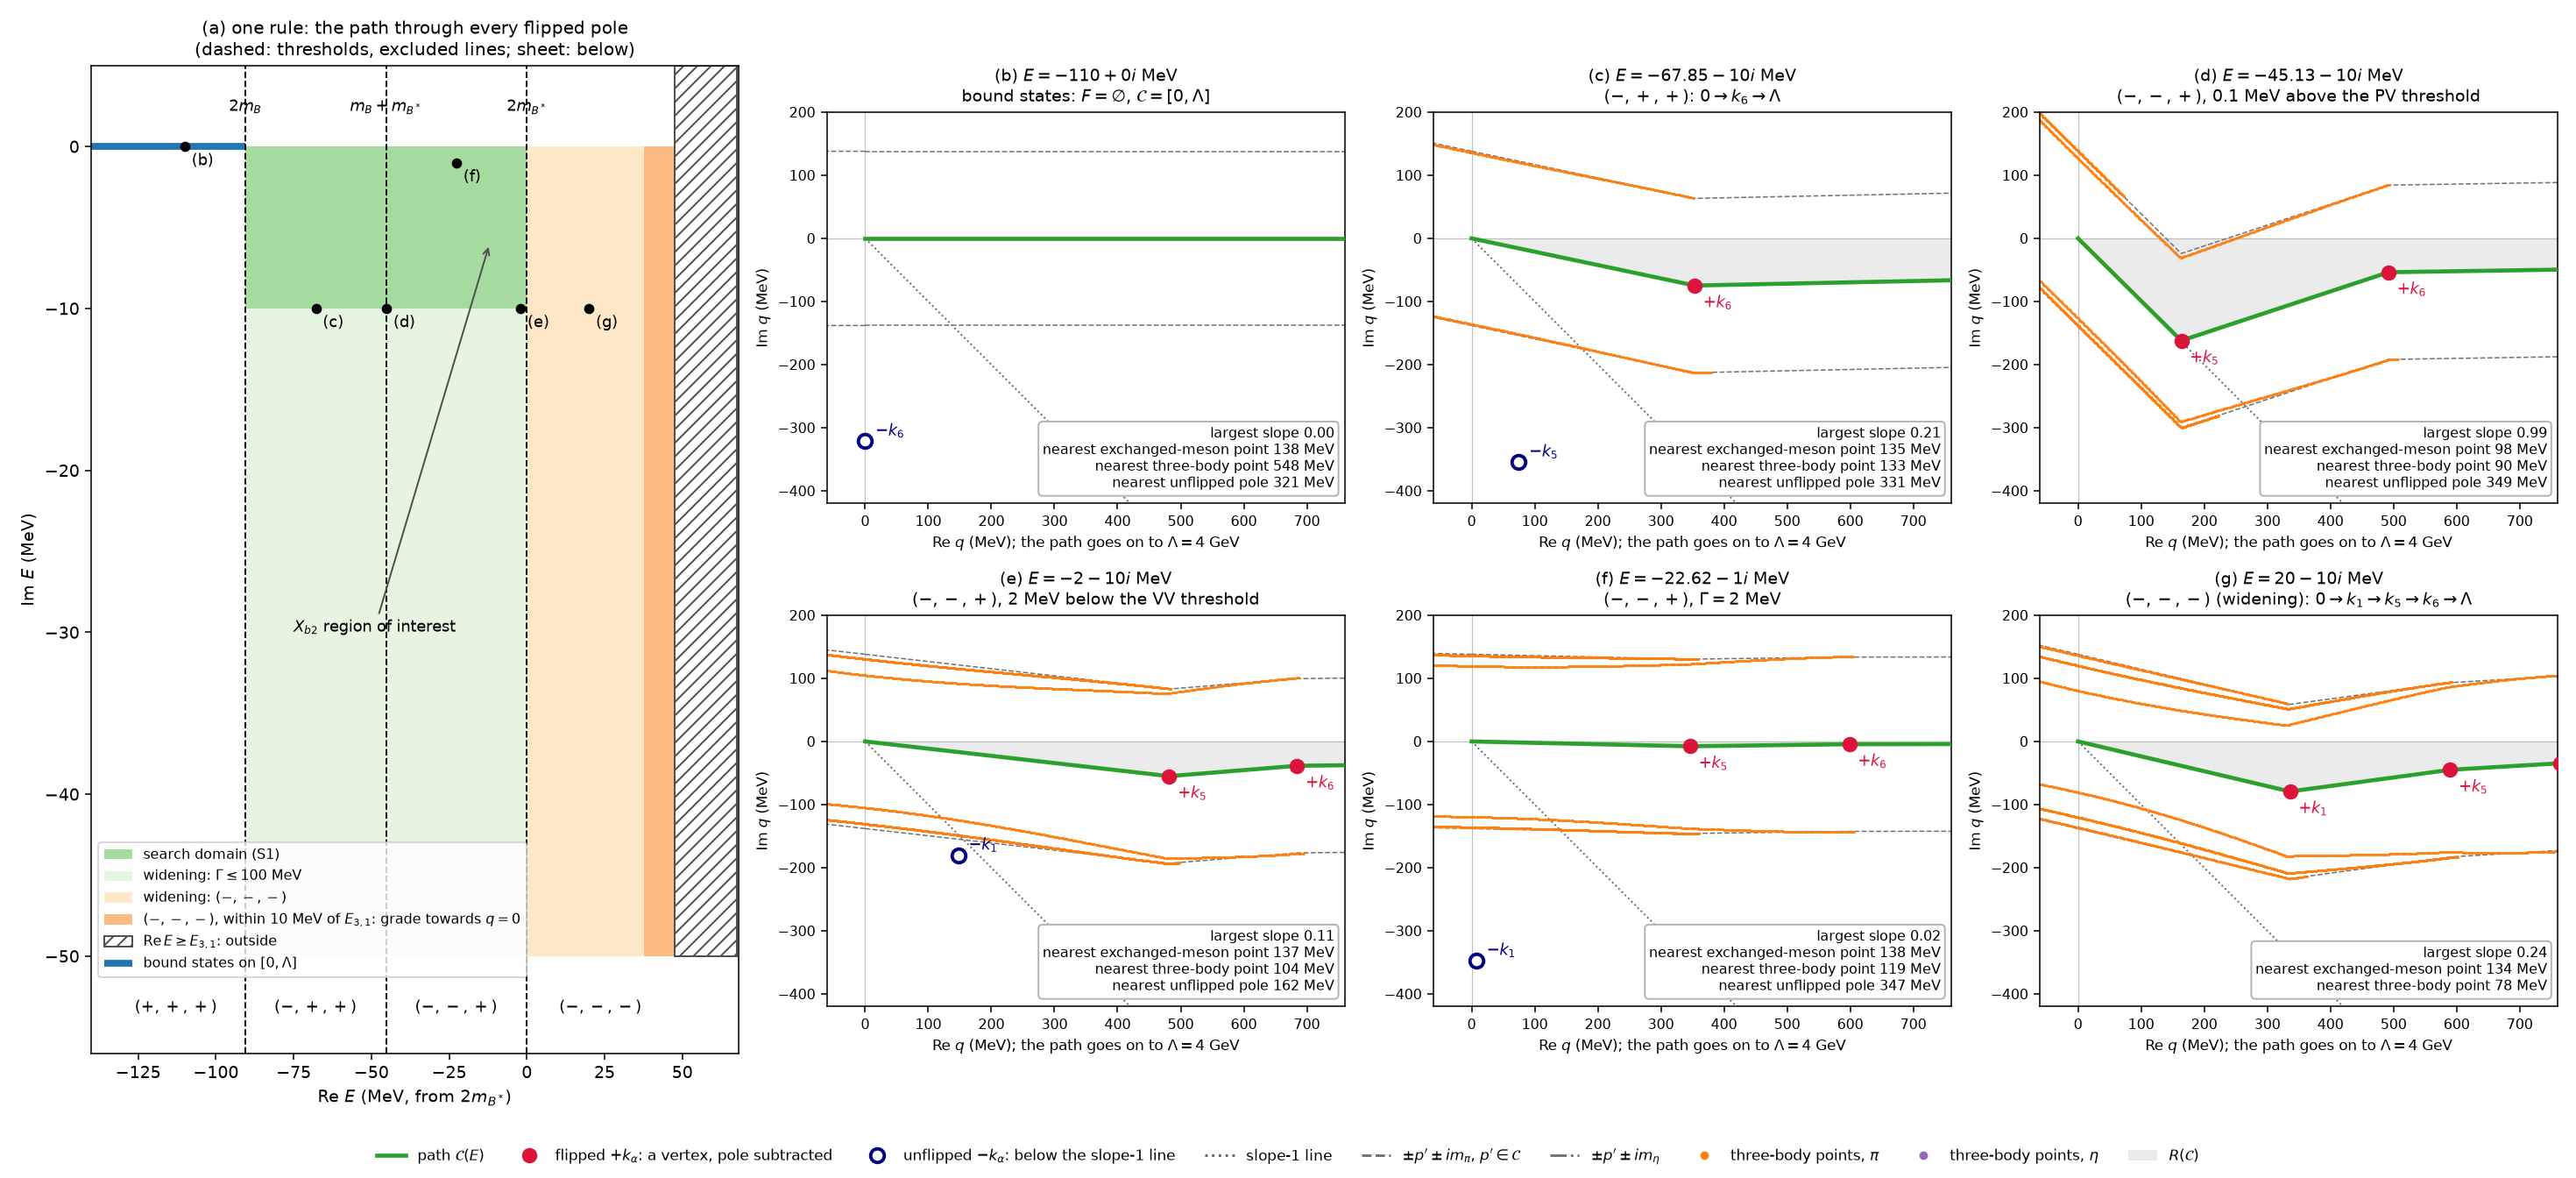
\includegraphics[width=\textwidth]{sp_rule.png}
\caption{The rule region by region. (a) The energy plane: search domain, widenings, excluded lines and the region outside. (b)--(g) $\mathcal C(E)$ at one probe energy per scenario, with the singular points of $V(p',q;E)$ for $p'\in\mathcal C$.}
\label{fig:rule}
\end{figure}

\begin{figure}[ht]
\centering
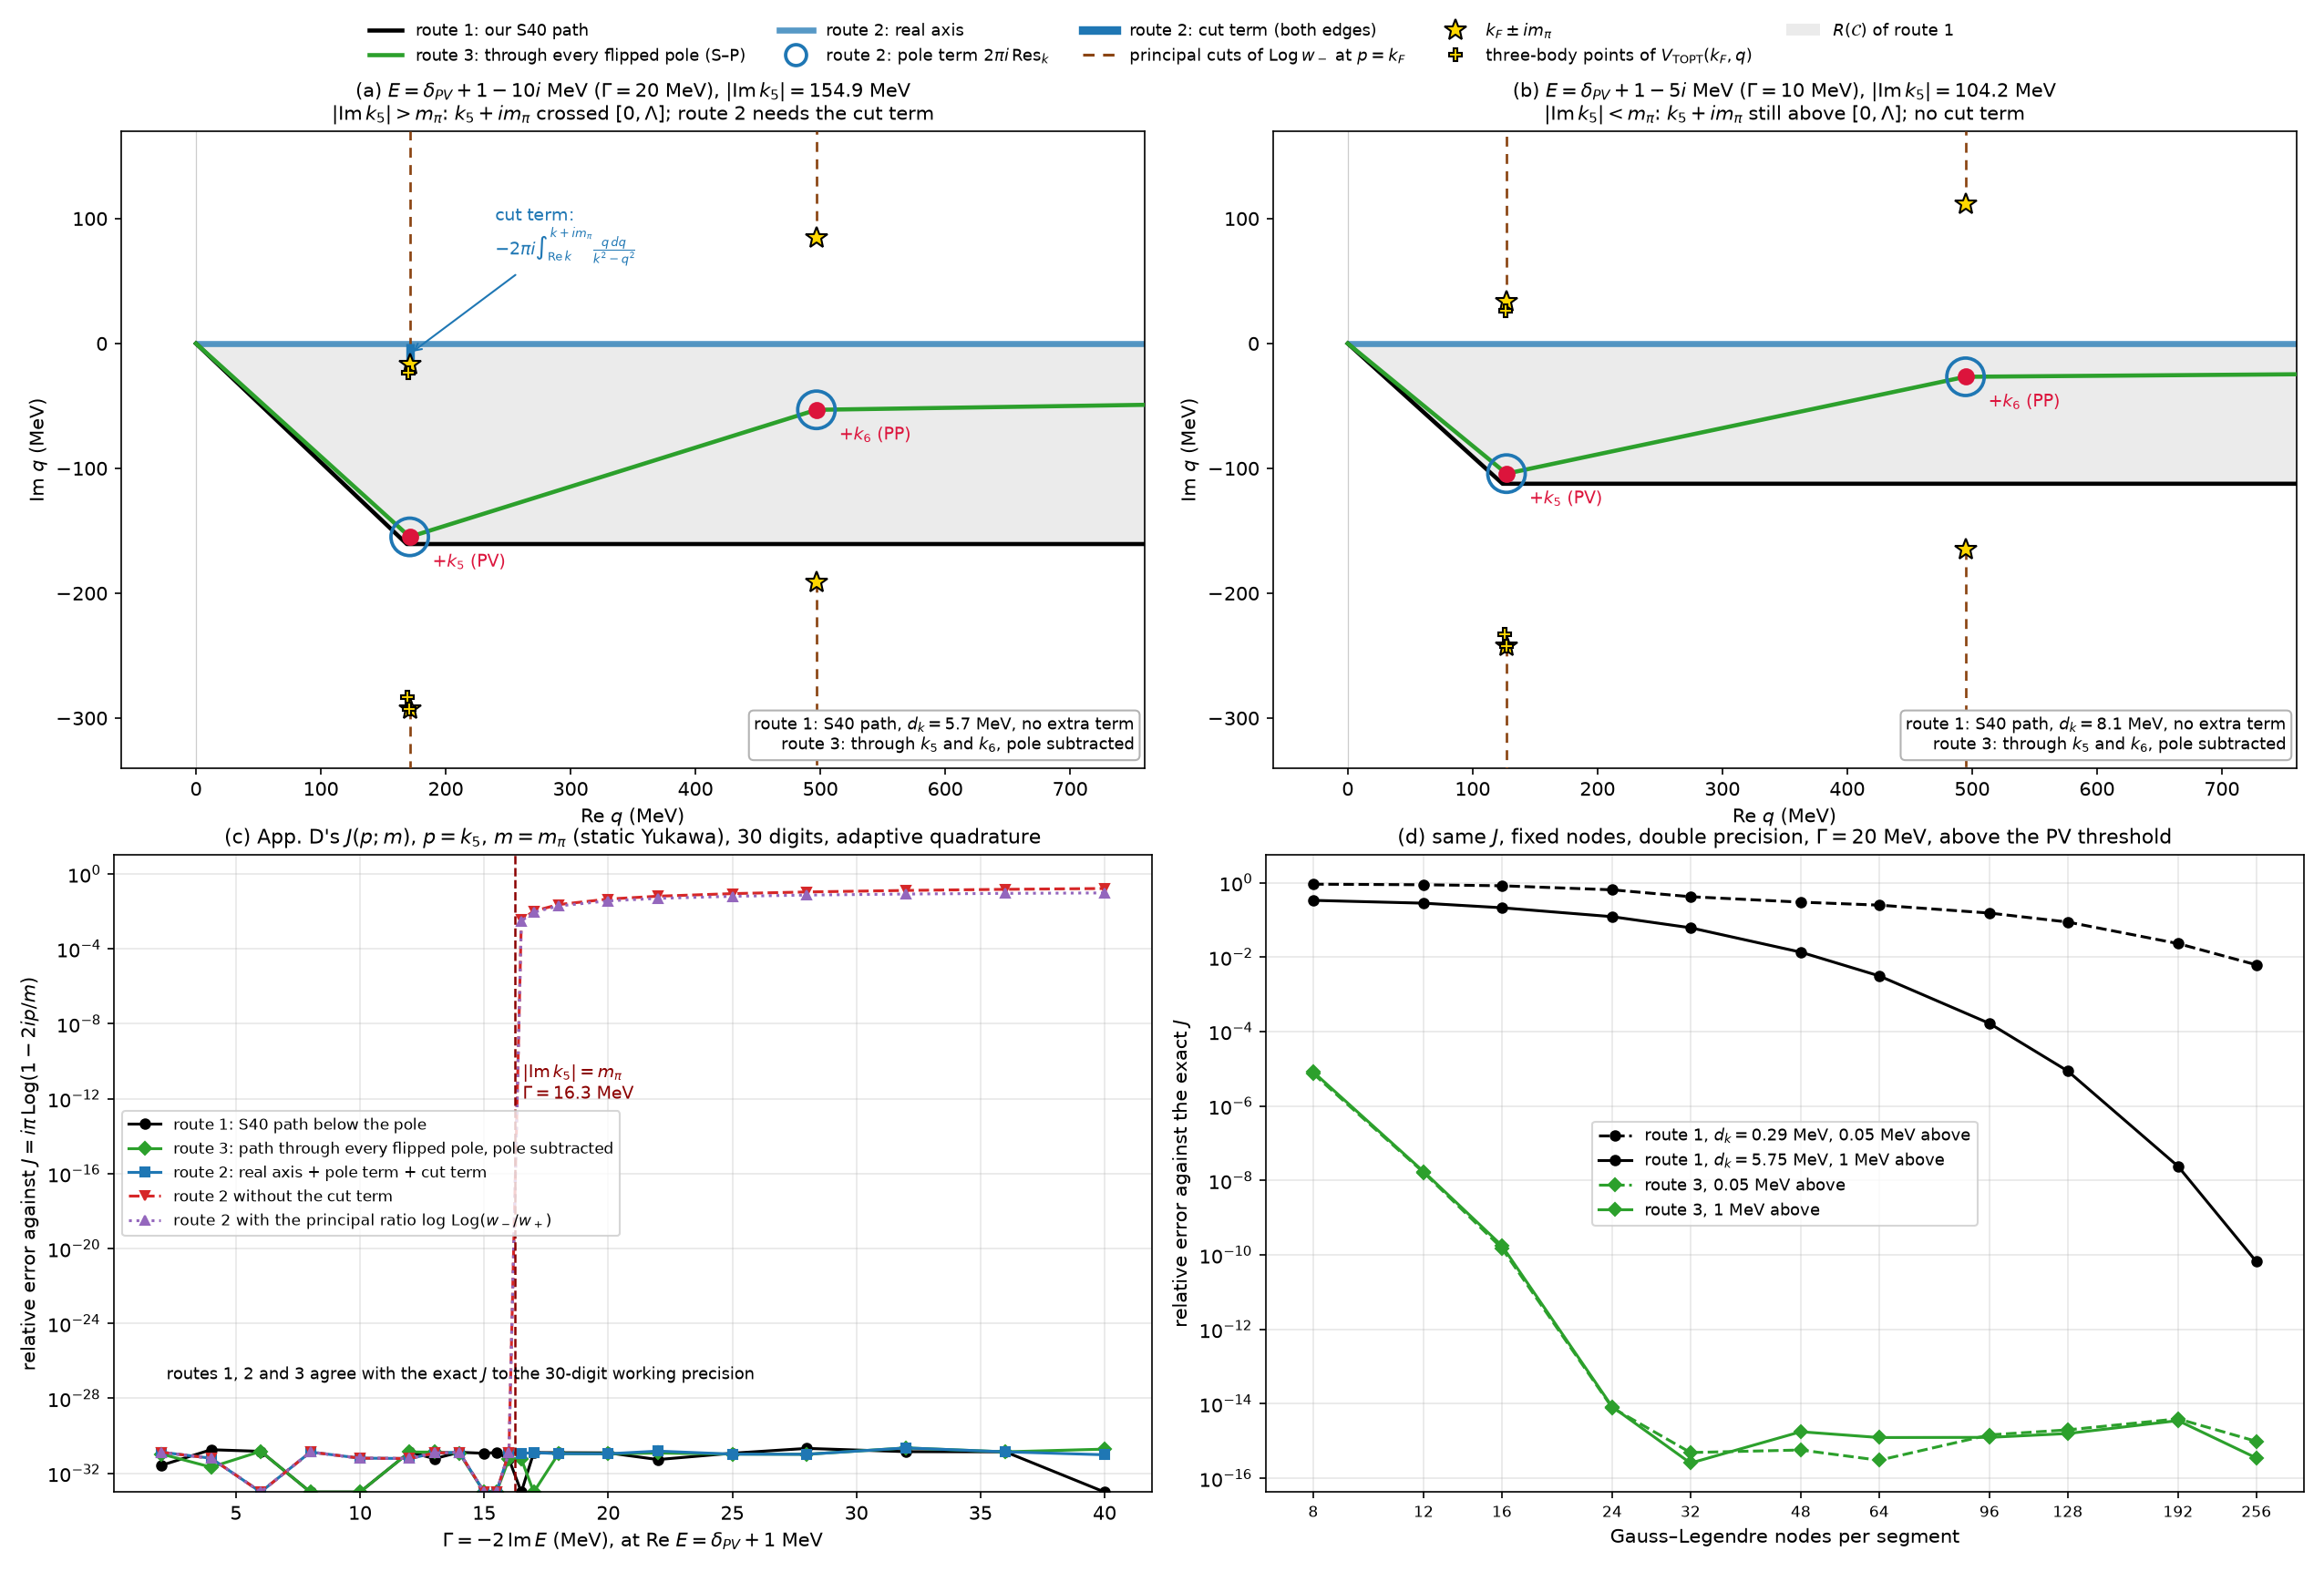
\includegraphics[width=\textwidth]{onshell_lhc_routes.png}
\caption{App.~D's $J$ with $p=k_5$: route 1, the S40 path; route 2, the real axis with pole and cut terms; route 3, the rule R1--R2.}
\label{fig:routes}
\end{figure}

\begin{figure}[ht]
\centering
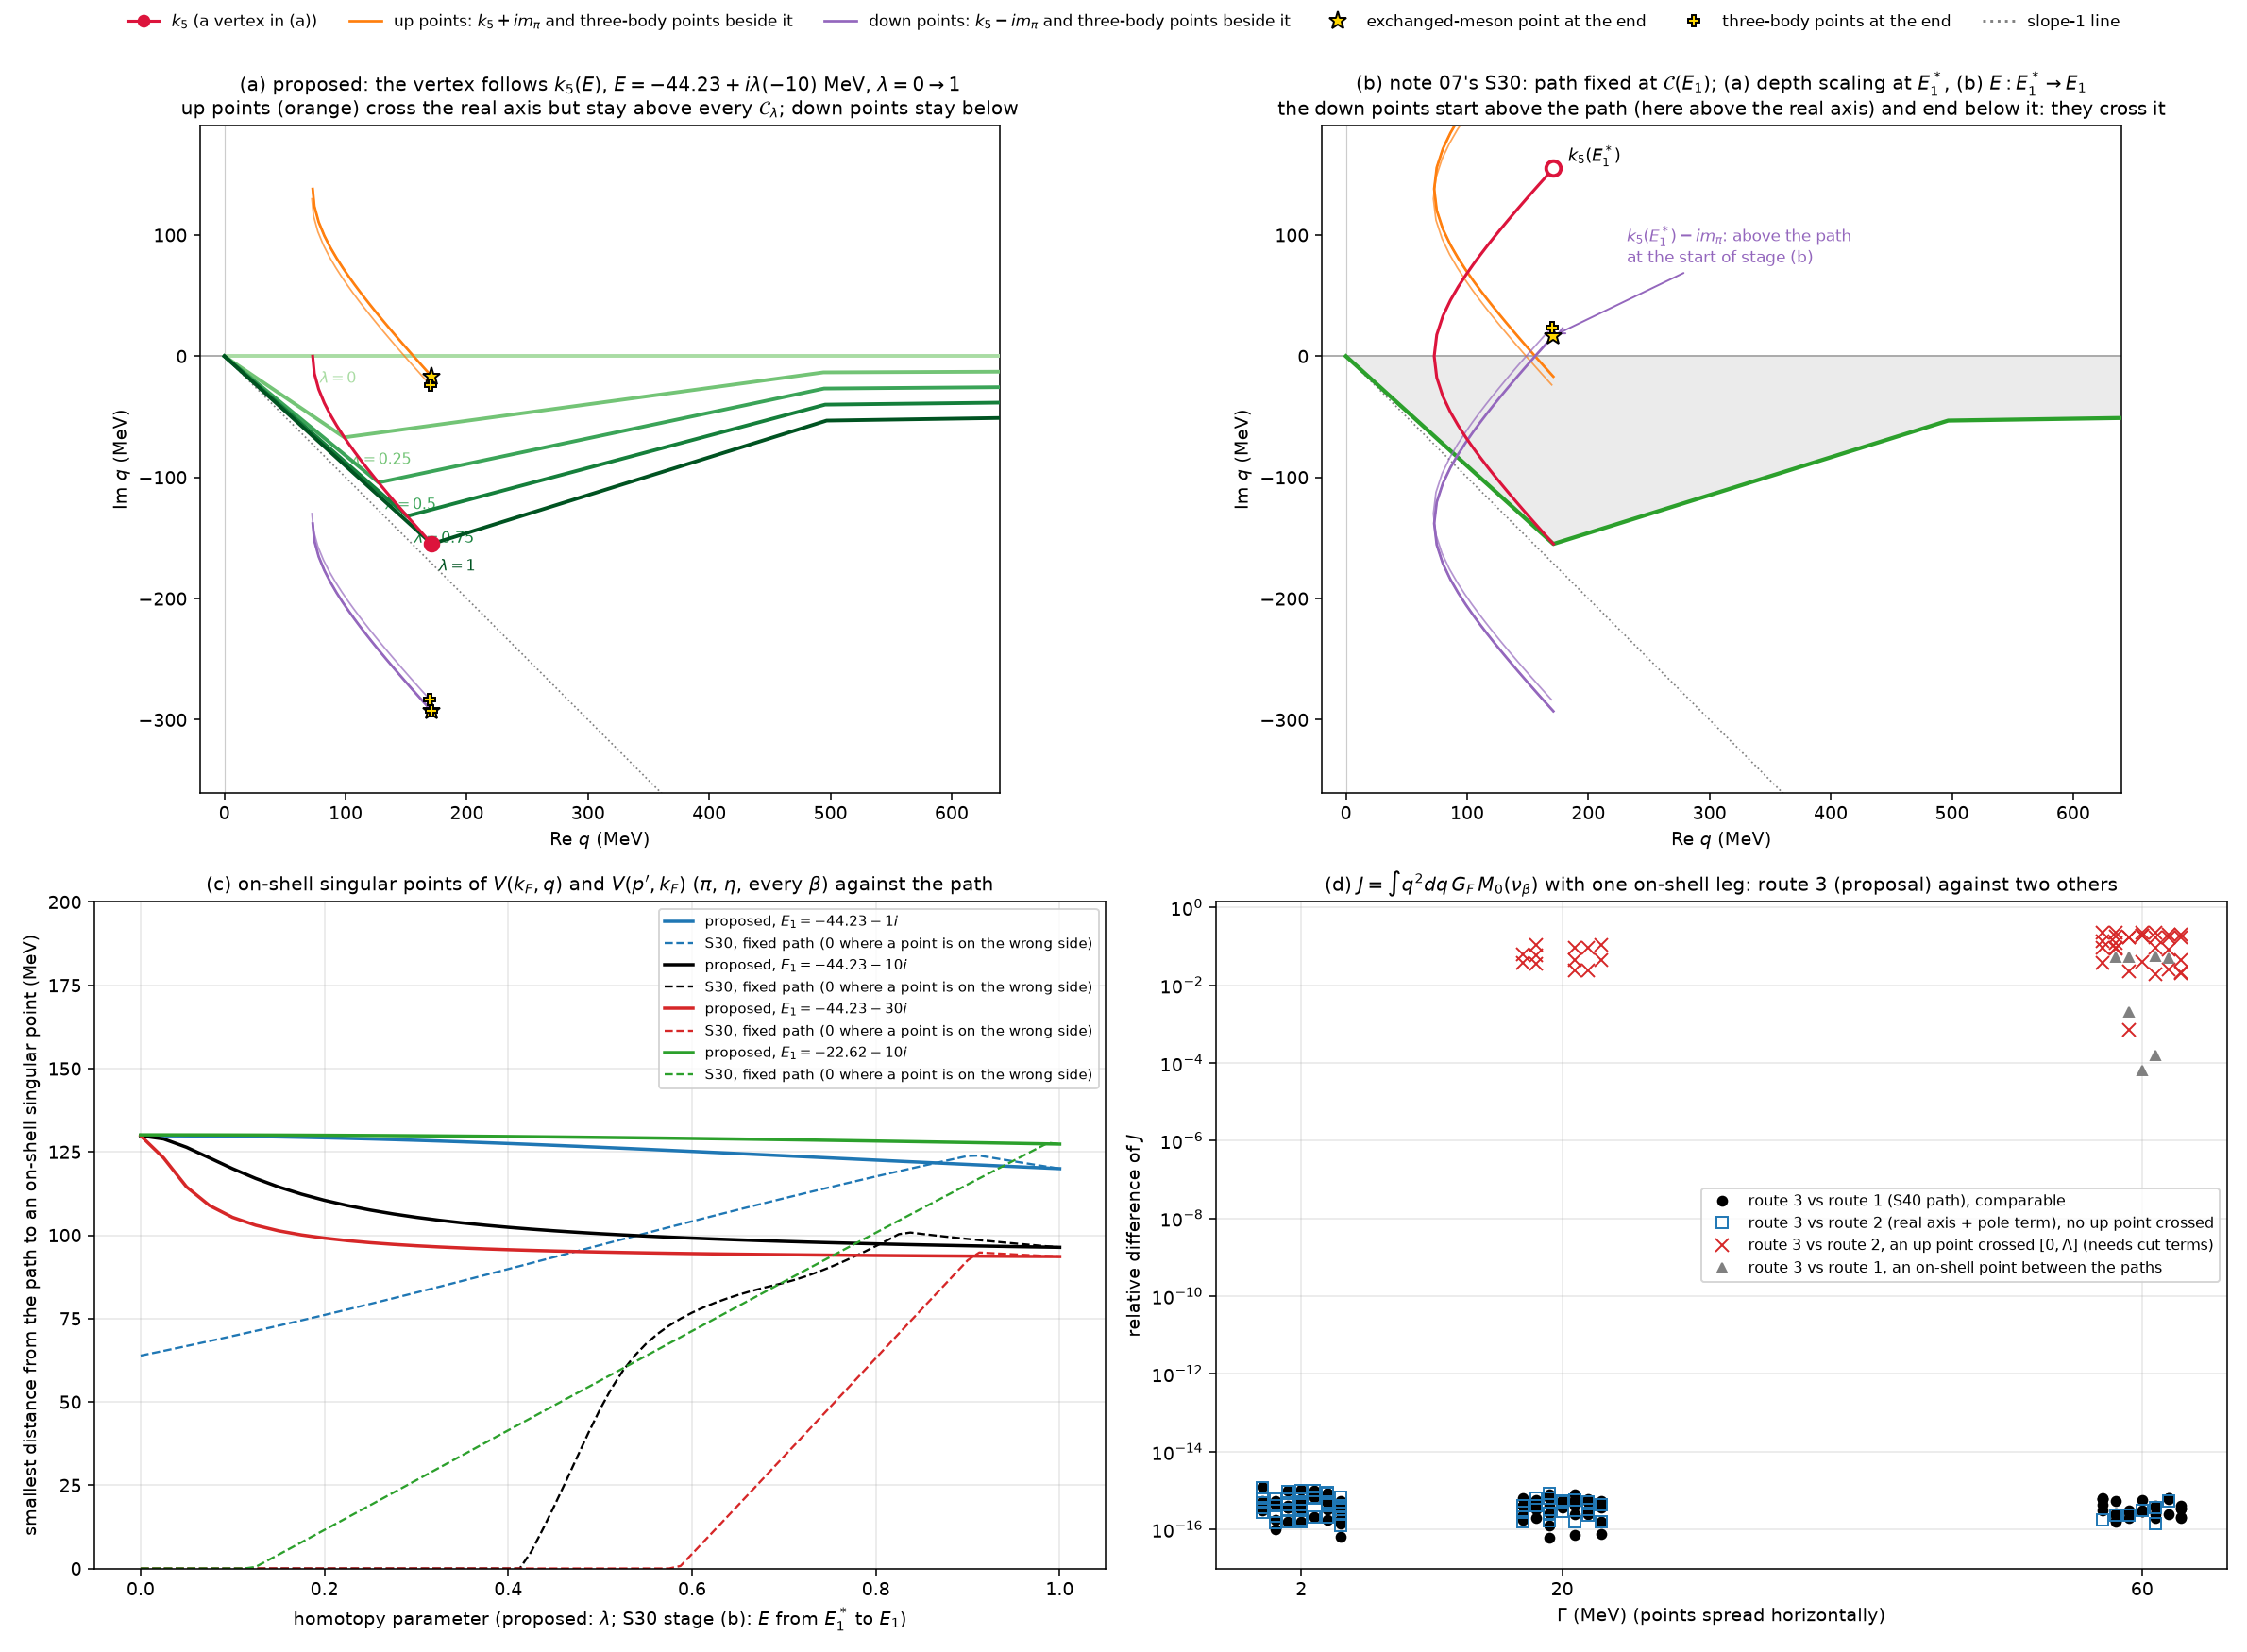
\includegraphics[width=\textwidth]{onshell_topt.png}
\caption{The on-shell node. (a) Along $\mathcal H$ at $E_1=-44.23-10i$~MeV the vertex follows $k_5$; up points cross the real axis but stay above every $\mathcal C_\lambda$, down points stay below. (b) S30's fixed path: the down points start above it and end below it. (c) Distance from the path to the on-shell singular points along both homotopies. (d) $J$ with one on-shell TOPT leg: route~3 against routes~1 and~2.}
\label{fig:topt}
\end{figure}

\section{Sheet as a sign}\label{sec:sign}

The rule adopted by the user on 2026-11-13 (note~07, S40) chooses a fixed certified path per rectangle. Its geometry serves kernel analyticity, including at the on-shell rows and columns. The polygon of R1 establishes the continuation on the adjacent strips; it does not prescribe the shape of the path. With Sokhotski--Plemelj subtraction the sheet enters a node channel $\alpha$ only through the sign $\sigma_\alpha$ in
\[
I_\pm(k)=\frac1{2k}\Bigl[\operatorname{Log}\frac{\Lambda-k}{\Lambda+k}\pm i\pi\Bigr],
\]
$+$ for the value with the analytic integral passing below $k_\alpha$ (flipped), $-$ for above it (unflipped); $k_\alpha$ is the principal root, in the fourth quadrant. For a channel treated by subtraction the actual path may pass on either side of its propagator pole or through it. In all three cases the node is at $k_\alpha$ with the weight of Eq.~\eqref{eq:W}, $I$ replaced by $I_{\sigma_\alpha}$. When the actual path passes on the sheet's side, the correction vanishes in the continuum. For a channel not treated by subtraction the path still has to pass on the sheet's side.

\paragraph{Valid paths.} For $\operatorname{Im}E<0$, $\operatorname{Re}E<E_{3,1}$ and a sheet $\sigma$, $\mathcal V(E,\sigma)$ is the set of graph paths in the closed lower half-plane with slopes at most $1$ such that
(i)~for every flipped channel the up points of $V(k_\alpha,q)$, $k_\alpha+im_\phi$ and the three-body points beside it, lie above the path, and
(ii)~for every unflipped channel the down points, $k_\alpha-im_\phi$ and those beside it, lie below the path.
On-shell $T$ at a node needs in addition the other side of that channel, the window of L5. A path that passes $k_\alpha$ on the side the sheet asks for meets (i) or (ii) by itself, because the up points lie above $k_\alpha$ and the down points below. So the conditions bind only for poles passed on the other side, where they are the windows of the nodes. Condition (ii) holds for every unflipped channel below its threshold, whose down points lie below the slope-1 line (L2).

\paragraph{L7: one value per sheet.} $\mathcal V(E,\sigma)$ is convex, and $D^\sigma_{\mathcal C}(E)$ is the same for every $\mathcal C\in\mathcal V(E,\sigma)$.

\emph{Proof.} Each condition is linear in $h$: $|h(x)-h(y)|\le|x-y|$, $h\le0$, and $h(\operatorname{Re}z)<\operatorname{Im}z$ or $h(\operatorname{Re}z)>\operatorname{Im}z$ for each listed point $z$. So $h_t=(1-t)h_0+th_1$ stays in $\mathcal V$. In the continuum the system on $\mathcal C_t$ with its nodes equals the plain system on $\mathcal C_t$ indented by a small $\epsilon$ to the side $\sigma_\alpha$ of each pole it passes on the other side. The subtracted integrand is regular at $k_\alpha$, and $\int_{\mathcal C_t}dq/(q^2-k_\alpha^2)$ differs from $I_{\sigma_\alpha}(k_\alpha)$ by exactly the residue term. When $\mathcal C_t$ crosses $k_\alpha$, the node switches on or off and the total stays continuous. On the indented path the kernel is analytic: the moving singular points stay off it by S34 and S35 (slopes at most $1$; the small indentation by continuity), and the fixed points of the nodes in use by (i) and (ii). S25 keeps $D$ constant in $t$. $\square$

\paragraph{Continuation.} For a fixed path, $E\mapsto D^\sigma_{\mathcal C}(E)$ is analytic where $\mathcal C\in\mathcal V(E,\sigma)$ (L6). The conditions are strict inequalities, so every $E$ with $\mathcal V(E,\sigma)\ne\emptyset$ has a neighbourhood on which one path stays valid. By L7 these local functions agree on overlaps and form one analytic function on $R_\sigma=\{E:\mathcal V(E,\sigma)\ne\emptyset\}$. On the adjacent strip of $\sigma$ the polygon of R1 lies in $\mathcal V$ (L5) and gives the continuation (L3). On the part of $R_\sigma$ connected to that strip, the identity theorem makes $D^\sigma$ the continuation within $\operatorname{Im}E<0$. That part includes hidden poles, the threshold lines, and the strip just below the highest flipped threshold.

\paragraph{L8: node pairs on a rectangle.} Let $\mathcal C$ be a graph path with slopes at most $1$, $\alpha$ a node channel at energy $E$, $c_\alpha=\operatorname{Re}k_\alpha+ih(\operatorname{Re}k_\alpha)\in\mathcal C$ and $\Delta_\alpha=\operatorname{Im}k_\alpha-h(\operatorname{Re}k_\alpha)$. The node pairs are $(k_\alpha,q)$, $(q,k_\alpha)$, $q\in\mathcal C$, and $(k_\alpha,k_{\alpha'})$ with another node.
(a)~If $|\Delta_\alpha|<m_\phi$, no $w_\pm$ of a node pair reaches $(-\infty,0]$ along the depth scaling of S30 or along the segment from $c_\alpha$ to $k_\alpha$.
(b)~If, moreover, for every node pair the smaller value of $\operatorname{Re}s_\pm$ at the two ends of that segment plus the smaller value of $\operatorname{Re}\nu_\beta$ there is positive, then $\operatorname{Re}Z^{(\beta)}_\pm>0$ along both homotopies, and the principal values at the node pairs are their continuations from $\mathcal C\times\mathcal C$.
(c)~Where $\mathcal C$ passes $k_\alpha$ on the sheet's side, the continuum weight $W_\alpha$ vanishes, so the node's values do not enter $D$.

\emph{Proof.} (a)~Write $r=p'\mp q$. Depth scaling turns $r$ into $\operatorname{Re}r+i\lambda\operatorname{Im}r$, with $\operatorname{Im}w=2\lambda\operatorname{Re}r\operatorname{Im}r$, so the cut is reached only where $\operatorname{Re}r=0$. For $w_+$, and for two nodes with different real parts, that never happens; for $(k_\alpha,q)$ it happens only at $q=c_\alpha$, where $w_-=m_\phi^2-\lambda^2\Delta_\alpha^2>0$. Along the segment from $c_\alpha$ to $k_\alpha$, $\operatorname{Re}r$ is fixed and the same argument applies.
(b)~At fixed $x=\operatorname{Re}r$ write $u=(\operatorname{Im}r)^2$, so that $w=m^2+x^2-u+2ix\operatorname{Im}r$. Then $\partial_u(\operatorname{Re}s)^2=\tfrac12\bigl[(x^2-m^2+u)/|w|-1\bigr]\le0$, because $|w|^2-(x^2-m^2+u)^2=4m^2x^2\ge0$: $\operatorname{Re}s$ does not increase with $|\operatorname{Im}r|$. Under depth scaling $|\operatorname{Im}r|$ grows with $\lambda$, and $\operatorname{Re}p'^2$, $\operatorname{Re}q^2$ fall, so $\operatorname{Re}Z$ does not increase; it starts at $\operatorname{Re}Z\ge E_{3,\beta}-\operatorname{Re}E>0$ on real momenta and is smallest at the end. Along the segment, $\operatorname{Im}r$ is affine, so $|\operatorname{Im}r|$ is largest at an end and $\operatorname{Re}s$ is smallest there, while $\operatorname{Re}\nu_\beta$ is concave in the parameter, since $\operatorname{Re}p'^2=x_\alpha^2-(\operatorname{Im}p')^2$. Hence $\operatorname{Re}Z$ is bounded below by the stated sum on both homotopies, and $\operatorname{Log}Z$ never meets its cut. With (a), the principal values are the continuations. In the code, $(\operatorname{Re}s)^2=(|w|+\operatorname{Re}w)/2$ is bounded below through lower bounds of $\operatorname{Re}w$ and $|\operatorname{Im}w|$, on both of which it increases.
(c)~In the continuum $W_\alpha=2\mu_\alpha k_\alpha^2\bigl[I_{\sigma_\alpha}(k_\alpha)-\int_{\mathcal C}dq/(q^2-k_\alpha^2)\bigr]$, and the integral equals $I_{\sigma_\alpha}(k_\alpha)$ when $\mathcal C$ passes on the sheet's side. $\square$

\paragraph{Rectangles.} With the nodes $q_j$ and the node set $N_Q$ fixed on $Q$, every entry of the discrete system is analytic in $E$ on $Q$: $k_\alpha(E)$ and $W_\alpha(E)$ are, and the kernel is principal at every pair by S34, S35 and L8. Where $k_\alpha(E)^2=q_j^2$ the singularities of $G_\alpha(q_j)$ and $W_\alpha$ cancel in the determinant, because the subtracted combination is regular. At an energy in two certified rectangles, join the paths by $h_t=(1-t)h_0+th_1$. The slopes stay at most $1$, the depth stays at most the larger one, so S35 holds, and a pole on the sheet's side of both paths stays there. In L7 the continuum correction vanishes on the sheet's side; if the path crosses the pole, S34 and S35 apply at the crossing. Before it, the bounds of L8 along $h_t$ are bounded by their values at the two ends, by the same convexity and concavity. So L7 applies and both rectangles give the same continuum $D$. Values on shared edges agree in the continuum, and the certified rectangles of one sheet glue into one analytic function on each connected union. The reference polygon of R1 identifies that function with the continuation on an adjacent strip (L3, L5), whether or not either rectangle uses that polygon. Hence $D$ is the continuation on every certified rectangle connected to that strip. $\square$

\paragraph{One fixed-path candidate.} The tested polygon for a search rectangle with centre $E_c$ puts a vertex at $\operatorname{Re}k_\alpha(E_c)$, at depth $\min(|\operatorname{Im}k_\alpha|,\operatorname{Re}k_\alpha)$, for every flipped channel and every unflipped channel whose threshold lies below the rectangle's upper real-energy edge. The Julia reference uses this geometry; the C solver tries the real path first and uses this polygon as the starting shape for deformation trials only where the kernel bounds require them (note~07, S40(a)). The evidence below checks (i) and (ii) on a grid over the rectangle. The check uses only the masses, $m_\pi$, $m_\eta$ and the orderings: no low-energy constants, no $T$. In \file{sp_sheets.py} (Fig.~\ref{fig:sheets}), for $\Gamma\le60$~MeV on $(-,+,+)$, $(-,-,+)$ and $(-,-,-)$, this path is valid at every $\operatorname{Re}E$ above the highest flipped threshold. Below it, it stays valid down to $3$--$4$, $8$--$9$ and $14$--$15$~MeV at $\operatorname{Im}E=-0.5$, $-10.5$ and $-29.5$~MeV. Six rectangles of $81$ energies each, four of them across a threshold, show no failure. Further below, an up point of the channel flipped below its threshold lies under the slope-1 line, so no path with slopes at most $1$ passes below it, and $\mathcal V$ is empty. A steeper leg is then needed; S35 and L7 no longer apply, and the sampled validator of S38 takes over.

\paragraph{Evidence.} At $E=\delta_6-10i$, contours of slope $0.5$, $1$ and $1.5$ give App.~D's $J$ on $(-,+,+)$ and $(+,+,+)$ to $20$ digits. Eight energies, from the $B\bar B$ threshold line to hidden poles and $VV$ flipped below its threshold, agree with independent routes to $20$ digits for App.~D's $J$ and for the TOPT moment. On the straight-line family of Fig.~\ref{fig:window}, the interpolation of L7 for one integral, both stay exact across the whole window. No linear equation has been solved yet.

\paragraph{Tiling.} \file{code/Xb2Continuation/scripts/s40_tiling.jl} tiles the search domain and the widenings with certified rectangles (Fig.~\ref{fig:tiling}): cells of about $5\times5$~MeV, quartered where the certificate fails, down to $0.1$~MeV in the search domain, $0.5$~MeV for $\Gamma\le100$~MeV and $1$~MeV on $(-,-,-)$. With near nodes optional (note~07, S40(c), the user, 2026-11-15) the whole search domain is certified, in $29$ cells on each strip; the near node is dropped in $3$ cells on each, with the pole at least $53.9$~MeV from the path. Both strips are certified completely for $\Gamma\le100$~MeV, and on $(-,-,-)$ below $E_{3,1}$ $98.75\%$ at $\operatorname{Im}E\ge-10$~MeV and $87.8\%$ for $-50\le\operatorname{Im}E<-10$~MeV. On $(-,-,-)$ the S35 bound with its $H^2$ term fails, from $\operatorname{Re}E=33.9$~MeV at $\operatorname{Im}E=-50$~MeV up to $46.98$~MeV next to the axis; L4 has no such term.

Before near nodes were optional, two gaps remained in the search domain, just below a threshold, at the real axis: $\operatorname{Re}E\in[-47.14,-46.01]$, $\operatorname{Im}E\in[-0.70,0]$~MeV on $(-,+,+)$, and $[-1.91,-0.85]\times[-0.08,0]$~MeV on $(-,-,+)$ (Fig.~\ref{fig:gaps}). There the unflipped pole of that channel, $k_\alpha\approx-i\kappa_\alpha$, came within $r_{\rm near}$ of the path and became a node. Every path with slopes at most $1$ passes it on the sheet's side, so its weight vanishes in the continuum (L8(c)); the node serves accuracy only. The only pair that fails is the node pair $(k_\alpha,k_\alpha)$ with $s_+$ and pion exchange, where $w_+=m_\pi^2-4\kappa_\alpha^2$ on the axis. For $PV$ with $\beta=1$, $\operatorname{Re}\nu_1\approx-\Delta$ with $\Delta=m_{B^*}-m_B$, and C5 fails once $\operatorname{Re}s_+<\Delta$, i.e.\ for $\kappa_5>\sqrt{m_\pi^2-\Delta^2}/2=65.2$~MeV, $0.80$~MeV below the threshold. For $VV$ with $\beta=2$, $\operatorname{Re}\nu_2=0$ exactly, and C5 fails where $\operatorname{Re}s_+$ vanishes, next to the axis for $\kappa_1>m_\pi/2$, $0.89$~MeV below the threshold. These are the branch points of the on-shell left-hand cuts of one-pion exchange in the two channels, $k^2=-(m_\pi^2-\Delta^2)/4$ and $k^2=-m_\pi^2/4$. In the momentum plane, the three-body point and the exchanged-meson point of $V(k_\alpha,\cdot)$ that carry these cuts lie at $\operatorname{Re}q=-\operatorname{Re}k_\alpha$, a distance $2\operatorname{Re}k_\alpha$ from the node's vertical homotopy, and the distance vanishes on the real axis. Along that homotopy, at the sampled energies, $Z^{(\beta)}_+$ stays below the cut of the logarithm while $\operatorname{Im}E<0$, so the principal values there are still the continued ones. But $\operatorname{Re}Z<0$, which C5 cannot certify, and on the axis the pair lies on the cut. The gaps end where the pole leaves $r_{\rm near}=100$~MeV. With the node switched off (\file{gap_failures_fix.jl}, $r_{\rm near}=60$~MeV), all $100$ and $15$ excluded cells of the two gaps certify, with the pole at least $64.1$ and $67.1$~MeV from the path (plot evidence, not a recorded check). Dropping the node costs the quadrature error of the pole integral: on the starting panels, $1.1\times10^{-10}$ of the loop at $45$~MeV from the path and $1.4\times10^{-12}$ at $65$~MeV. For a channel flipped below its threshold the node cannot be dropped, since its residue is the continuation; there the same entry carries the on-shell left-hand cut into $D$ (note~07, S40(d); Stage~8). On $(-,-,-)$ the sampled smallest $\operatorname{Re}Z$ over pairs on the path equals the bound of L4, $E_{3,1}-\operatorname{Re}E$, while the $H^2$ term of S35 turns C2 negative from $\operatorname{Re}E\approx39$~MeV at $\operatorname{Im}E=-40$~MeV (Fig.~\ref{fig:s35h2}).

\begin{figure}[ht]
\centering
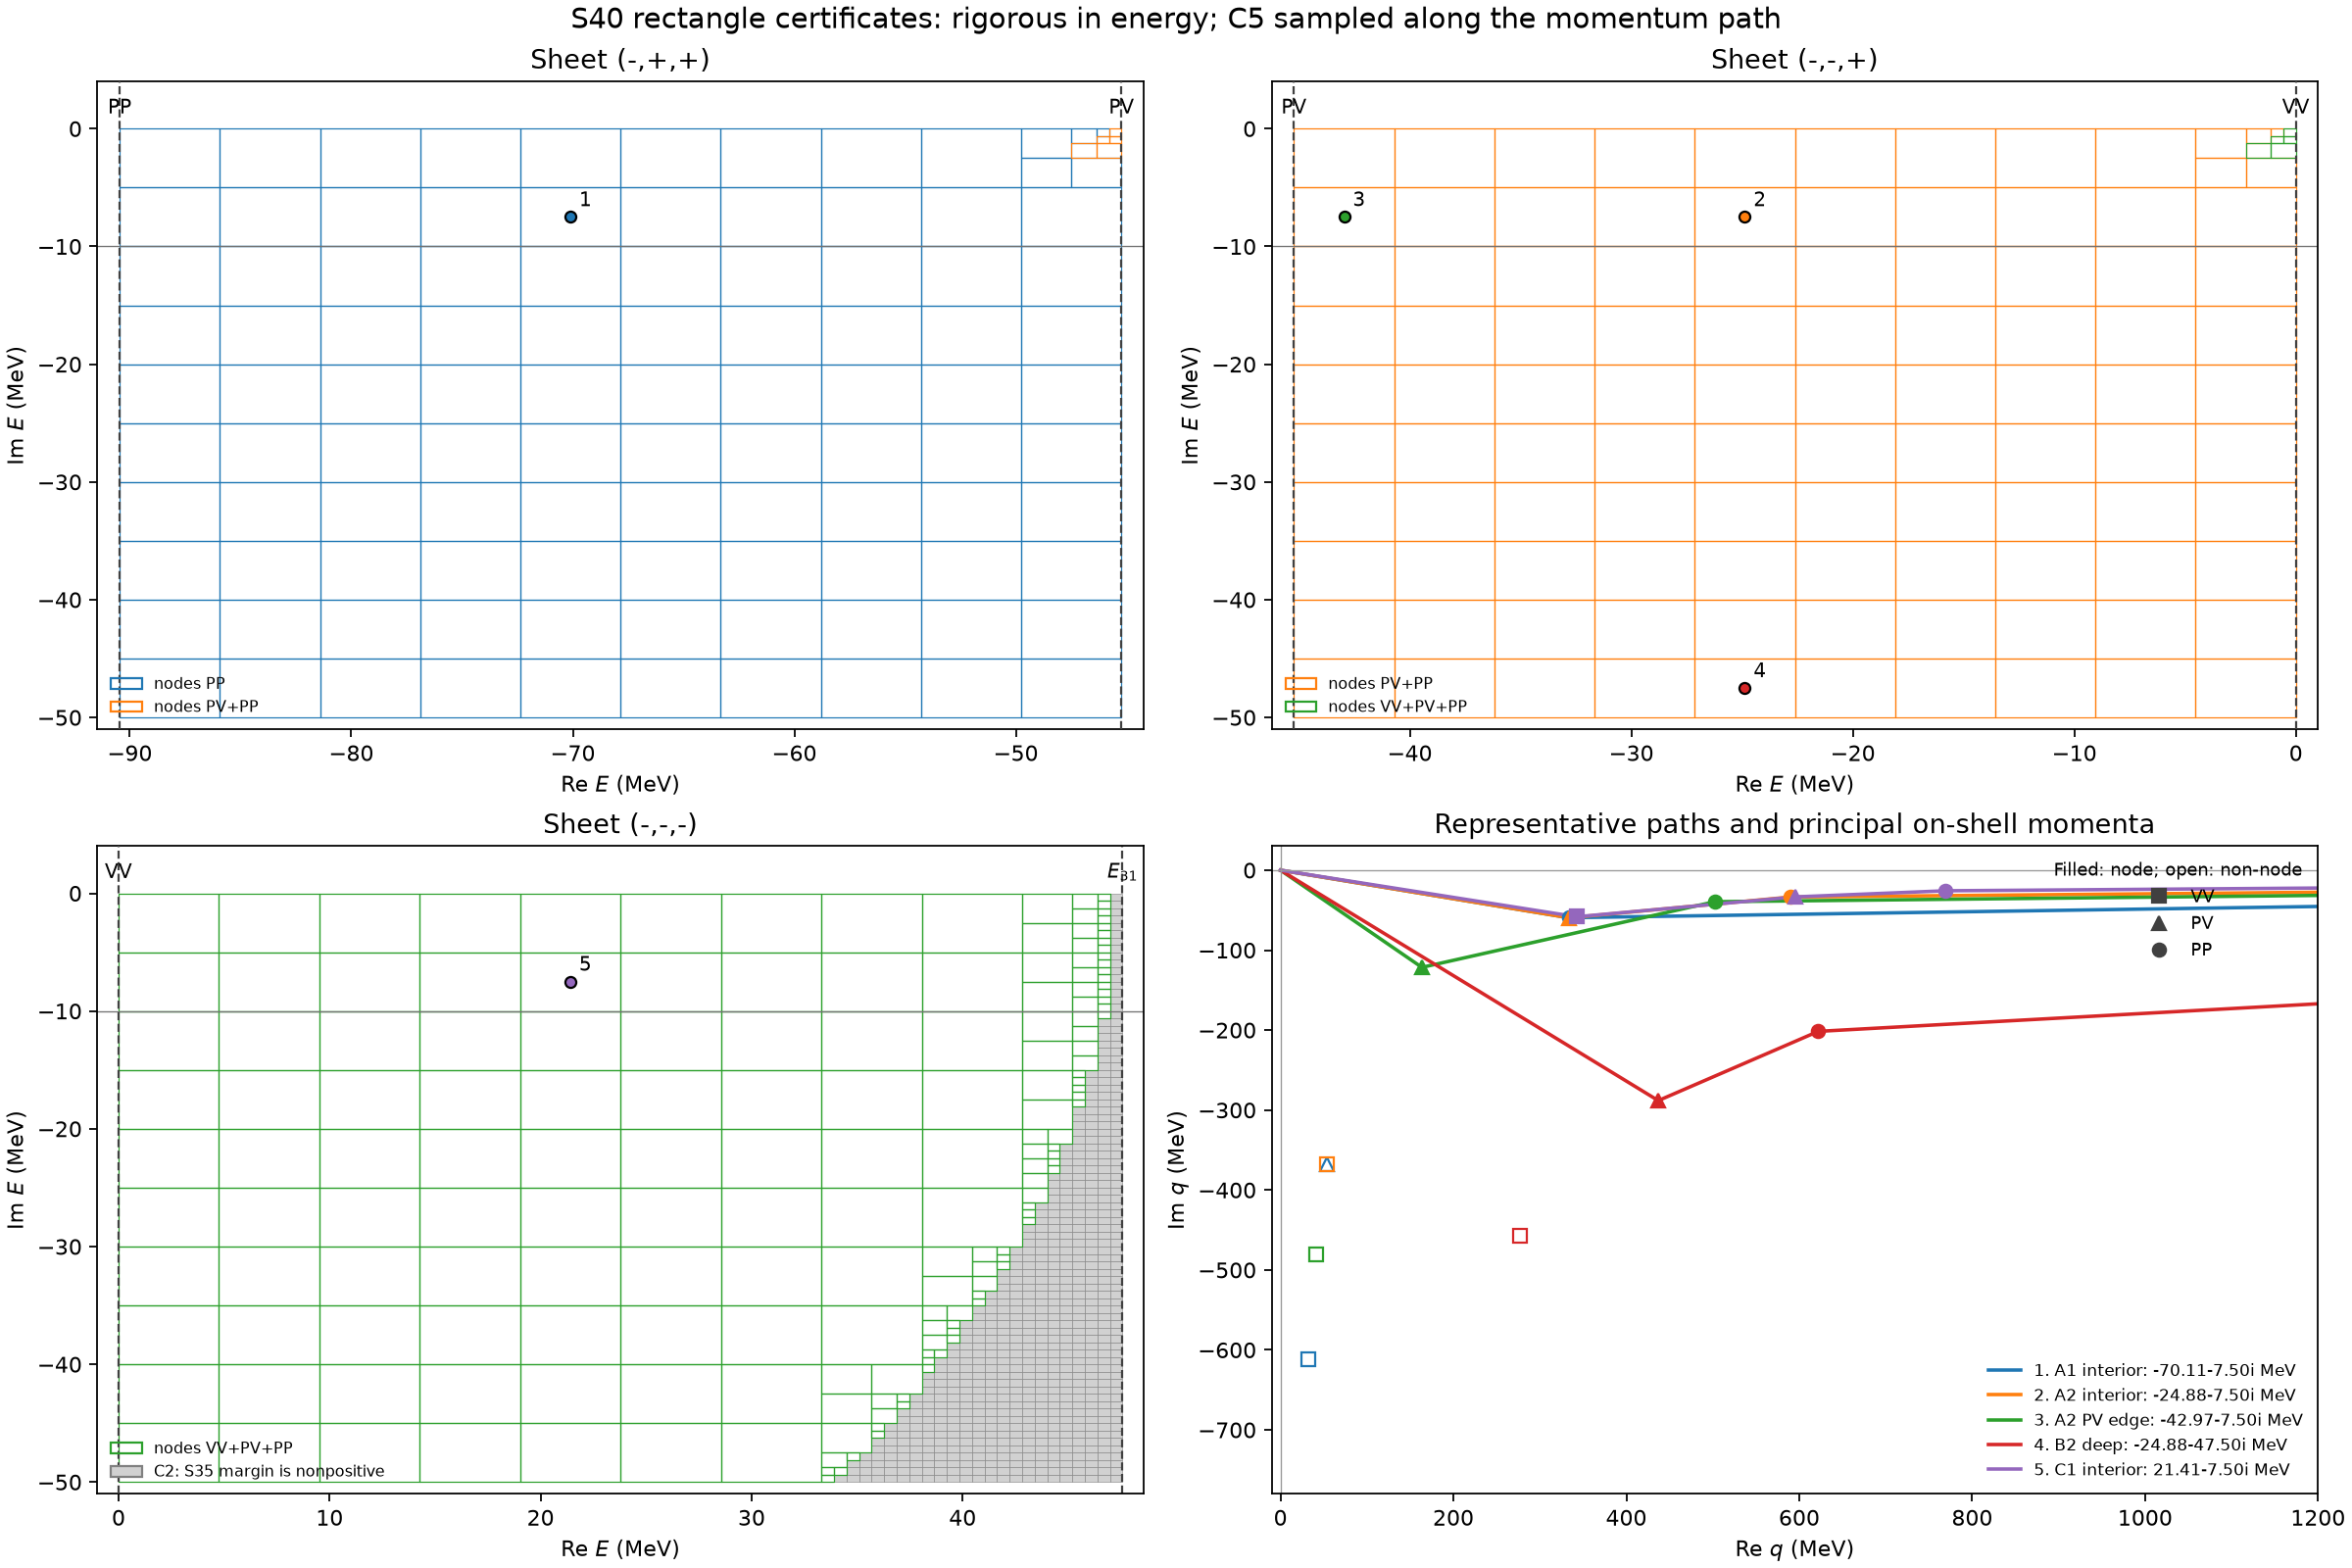
\includegraphics[width=\textwidth]{s40_tiling.png}
\caption{Certified rectangles (outlined, coloured by node set) and exclusions (grey) on $(-,+,+)$, $(-,-,+)$ and $(-,-,-)$, and the paths of five certified cells with the on-shell momenta at their centres (filled: node; open: not a node).}
\label{fig:tiling}
\end{figure}

\begin{figure}[ht]
\centering
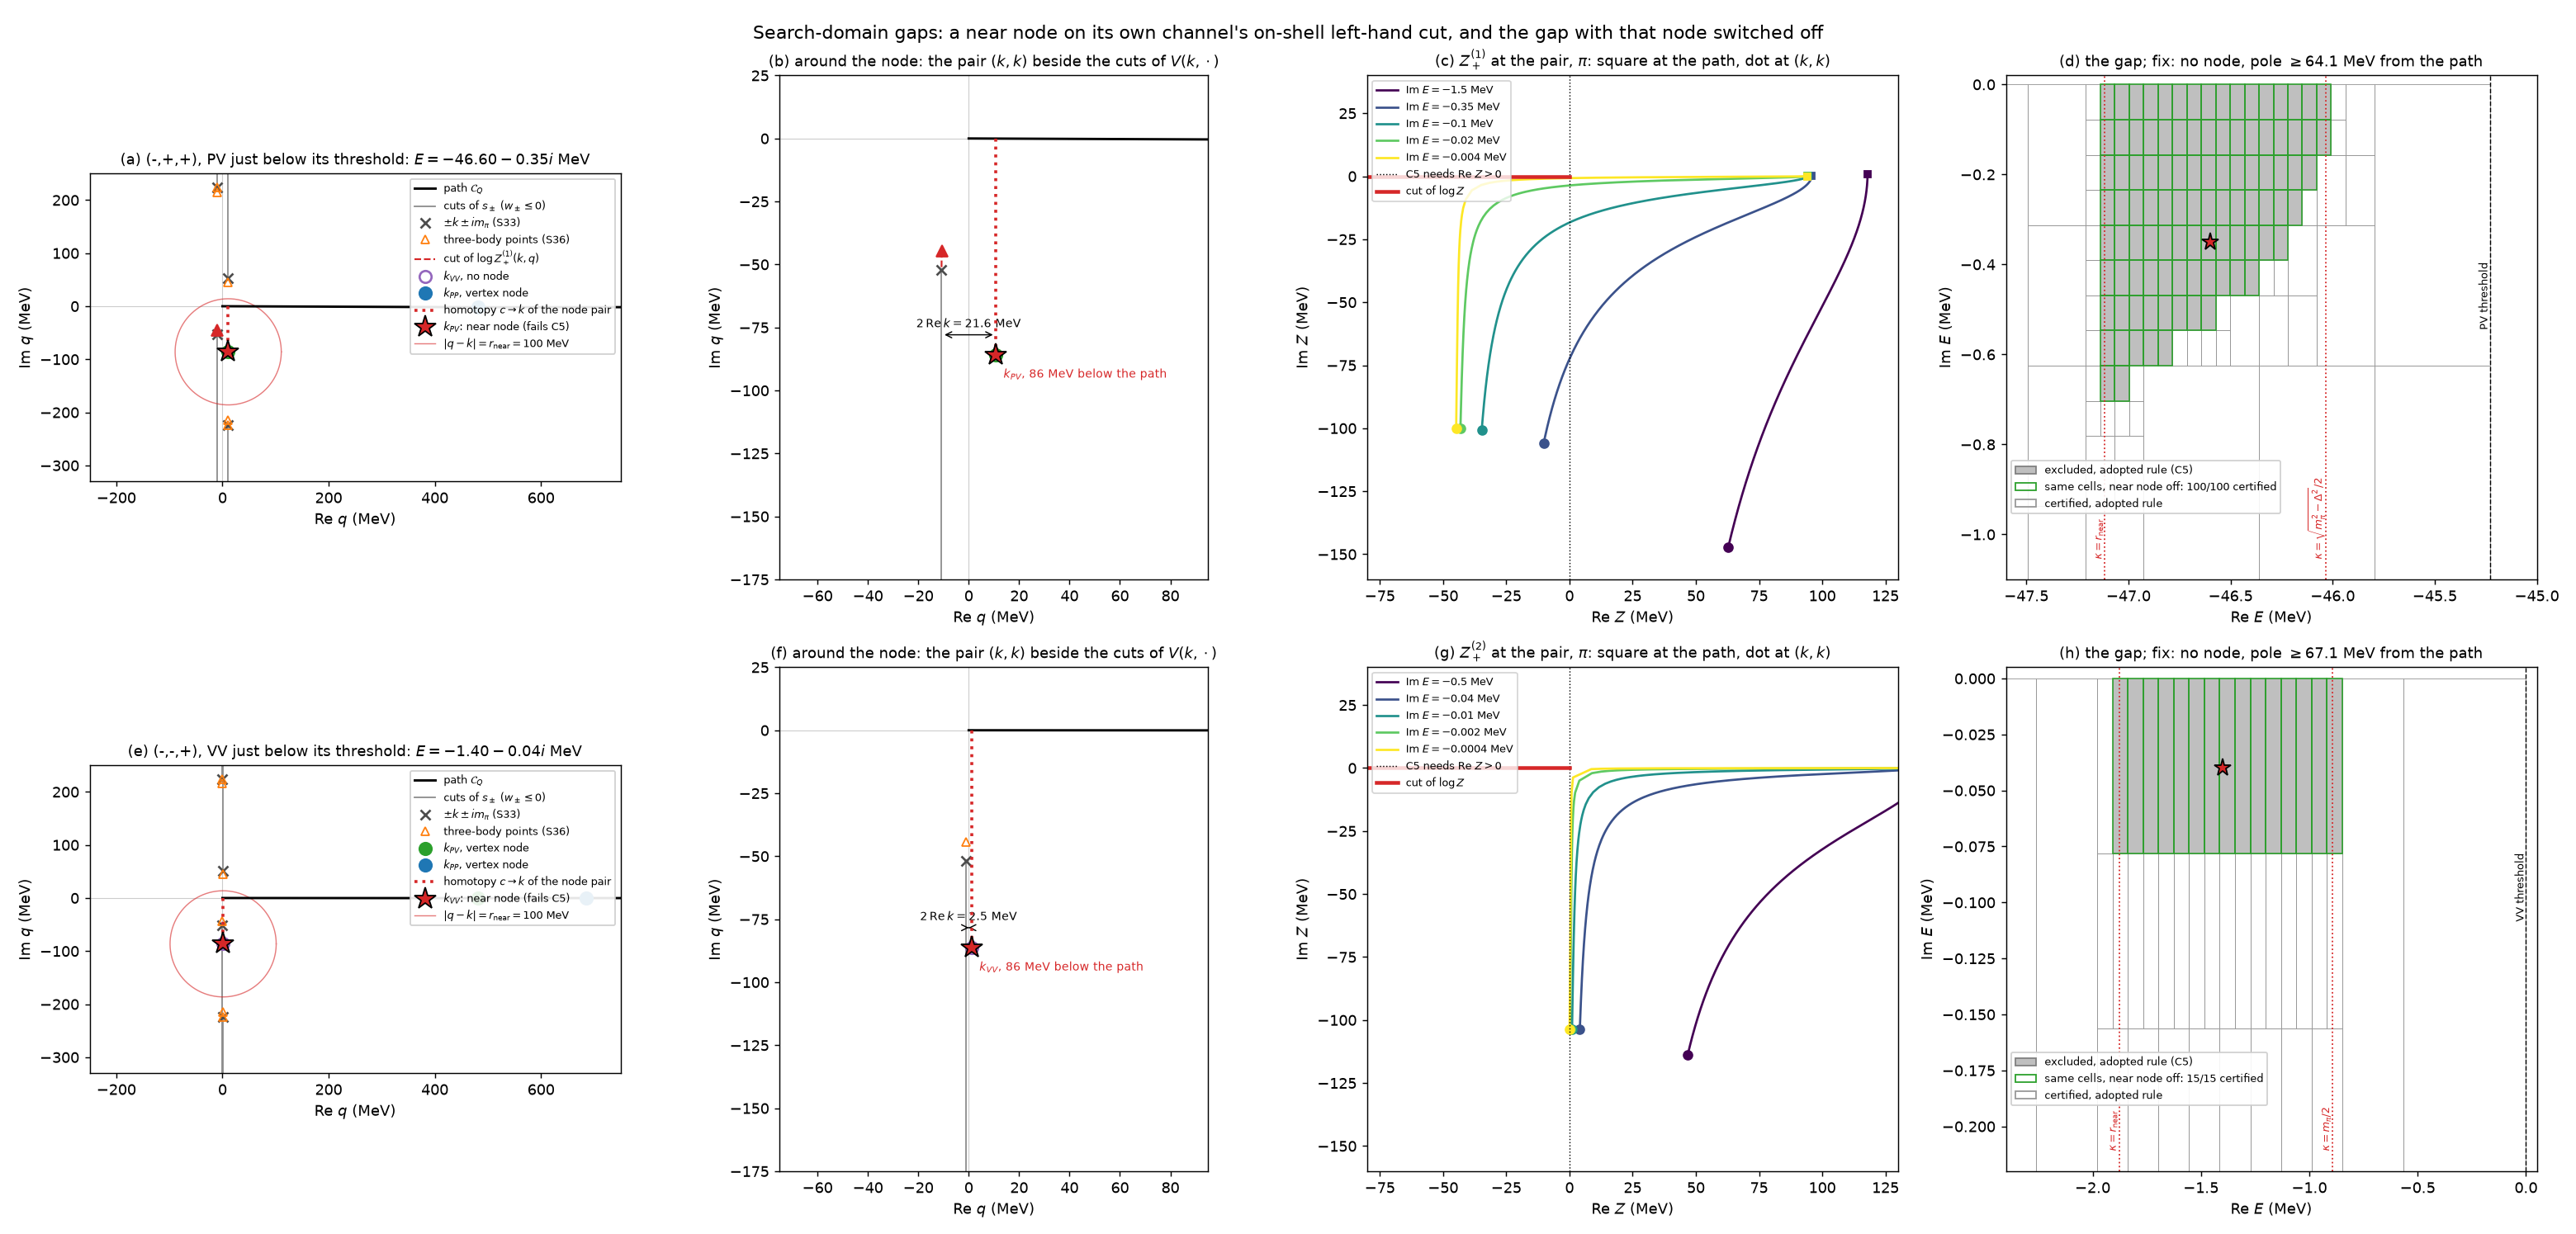
\includegraphics[width=\textwidth]{gap_failures.png}
\caption{The two search-domain gaps (rows). (a), (e) The path, the poles, and the near node that fails (red star), with the singular points of $V(k,\cdot)$ for pion exchange and the cuts of the failing pair. (b), (f) The same around the node: its vertical homotopy runs $2\operatorname{Re}k$ beside the cuts. (c), (g) $Z^{(\beta)}_+$ at the node pair along the homotopy that moves both momenta from the path to $k$, for several $\operatorname{Im}E$: C5 asks $\operatorname{Re}Z>0$. (d), (h) The gap cells under the adopted rule (grey) and the same cells with the near node switched off (green).}
\label{fig:gaps}
\end{figure}

\begin{figure}[ht]
\centering
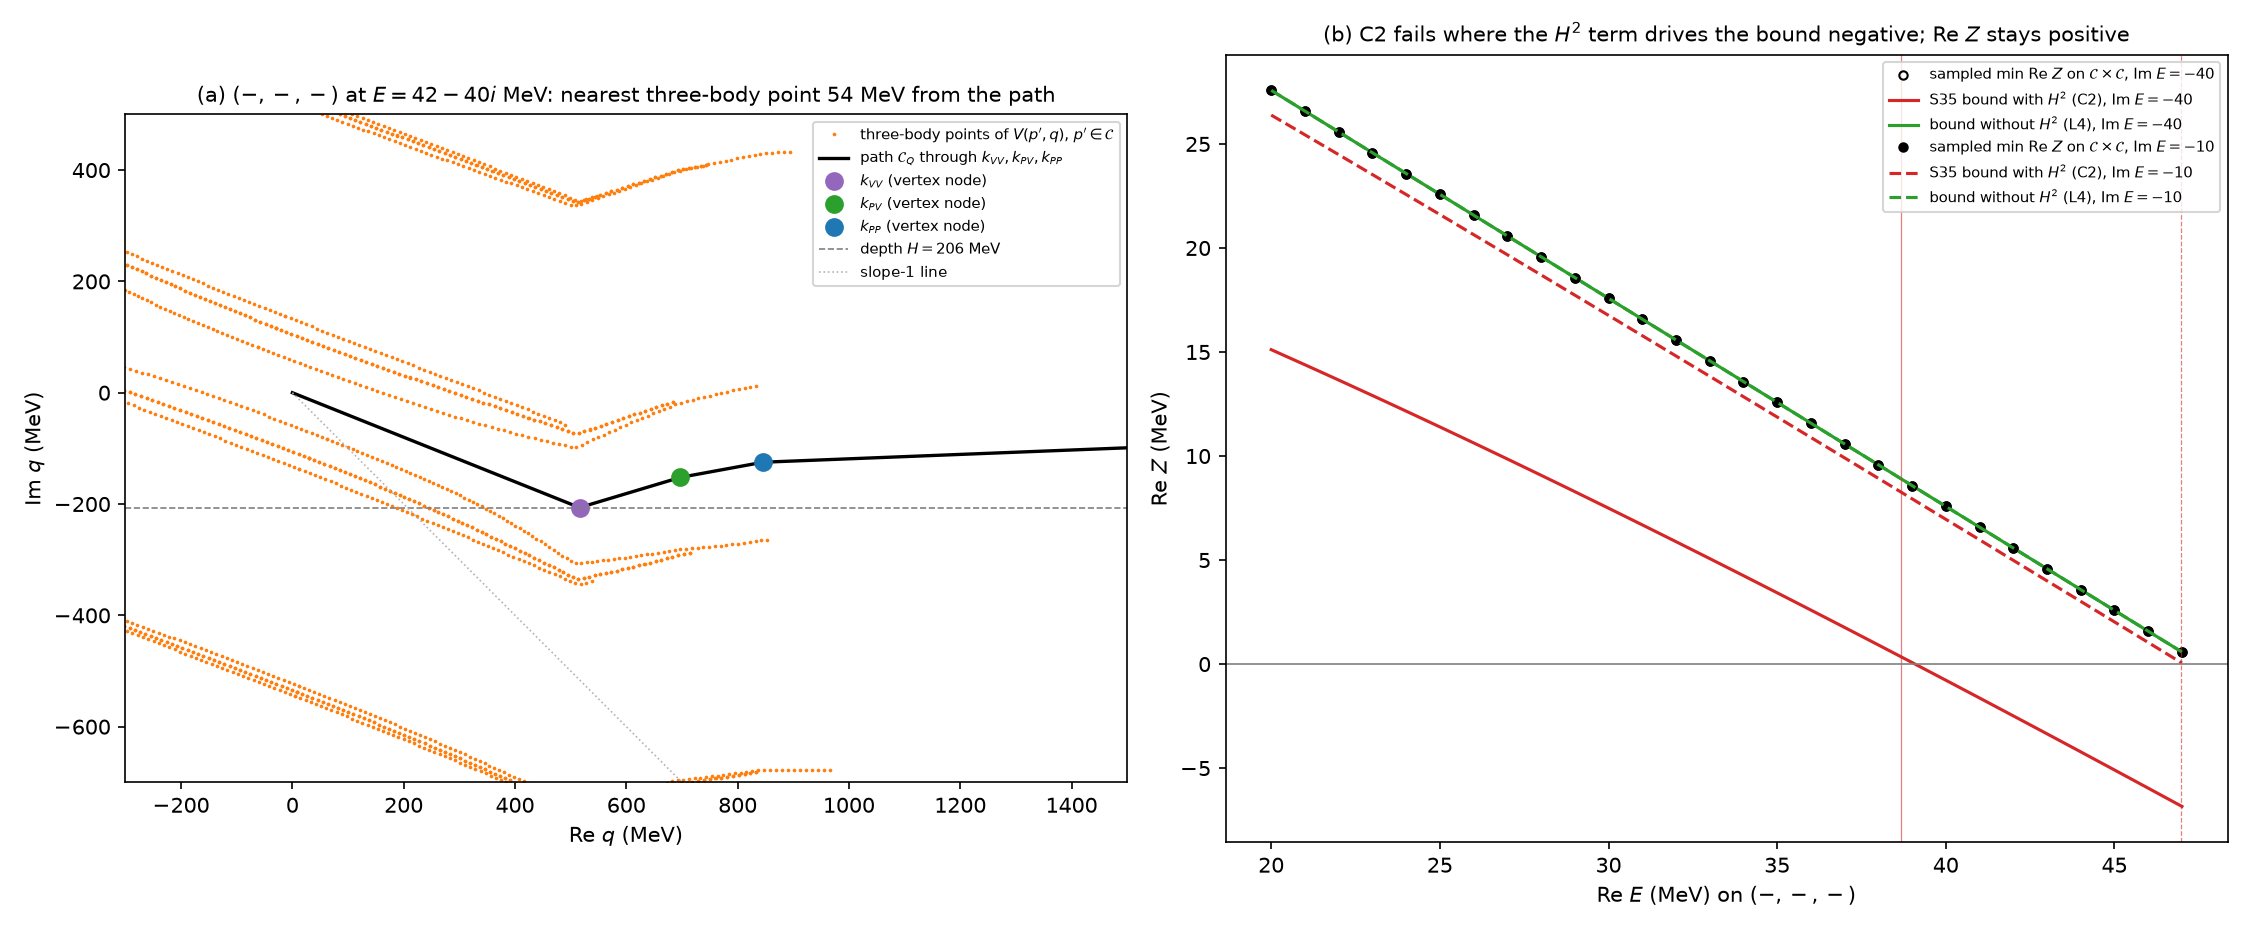
\includegraphics[width=\textwidth]{s35_h2.png}
\caption{The $(-,-,-)$ exclusions next to $E_{3,1}$. (a) The path at $E=42-40i$~MeV and the three-body points of $V(p',q)$ for $p'$ on it. (b) The sampled smallest $\operatorname{Re}Z$ over pairs on the path, the S35 bound with its $H^2$ term (C2) and the bound of L4, along $\operatorname{Im}E=-40$ and $-10$~MeV; vertical lines mark where the tiling starts to exclude.}
\label{fig:s35h2}
\end{figure}

\paragraph{The certificate in pictures.} Figures~\ref{fig:certpairs}--\ref{fig:certnodes} show what (C1)--(C5) of S40(d) ask, on certified rectangles and on cases that fail (\file{cert\_conditions.py}, with the certificates computed by \file{cert\_conditions.jl}; plot evidence, not a recorded check). Write $p'=x+ih(x)$ and $q=y+ih(y)$ for two points of the path.

\emph{(C1).} With slopes at most $1$ and $h(0)=0$, $|\operatorname{Im}(p'-q)|=|h(x)-h(y)|\le|x-y|$ and $|\operatorname{Im}(p'+q)|\le|h(x)|+|h(y)|\le x+y$: both $p'-q$ and $p'+q$ lie within $45^\circ$ of the real axis, their squares have a non-negative real part, and $\operatorname{Re}w_\pm\ge m_\phi^2$, $\operatorname{Re}s_\pm\ge m_\phi$ (S35). On the path of the rectangle $[-25,-20]\times[-50,-45]$~MeV on $(-,-,+)$, largest slope $0.63$, the smallest sampled $\operatorname{Re}w_\pm$ is $m_\pi^2$; on the steep probe path of Stage~2, whose first leg has slope $20$, it is $-7.4\,m_\pi^2$ (Fig.~\ref{fig:certpairs}(a), (b)).

\emph{(C2).} $\operatorname{Re}Z^{(\beta)}_\pm=\operatorname{Re}s_\pm+t_\beta+h_\beta\operatorname{Re}p'^2+a_\beta\operatorname{Re}q^2-\operatorname{Re}E$, with $\operatorname{Re}s_\pm\ge m_\phi$ by (C1) and $\operatorname{Re}p'^2=x^2-h(x)^2\ge-H^2$, gives $\operatorname{Re}Z\ge E_{3,\beta}-(h_\beta+a_\beta)H^2-\operatorname{Re}E$. On the same rectangle the certified bound is $52.6$~MeV and the smallest sampled value $67.6$~MeV, which is $E_{3,1}-\max\operatorname{Re}E$, taken at $p'=q=0$. On the steep path, at the rectangle's centre, $\operatorname{Re}Z$ falls to $-58$~MeV and $Z$ crosses the cut of the logarithm between neighbouring pairs: the principal kernel is discontinuous on that path (Fig.~\ref{fig:certpairs}(c)).

\emph{(C3).} A channel outside $N_Q$ is unflipped and below its threshold, so $\operatorname{Re}k_\alpha^2=2\mu_\alpha(\operatorname{Re}E-\delta_\alpha)<0$ and $|\operatorname{Im}k_\alpha|>\operatorname{Re}k_\alpha$: the pole lies under the line of slope $1$ through the origin, hence under every path with $|h(x)|\le x$, the side its sheet asks for. Its loop is the plain quadrature along the path, and the distance sets the error: for the $PV$ loop on $(-,+,+)$ with the starting panels, $3.5\times10^{-6}$ at $17$~MeV, $1.1\times10^{-10}$ at $45$~MeV, $1.5\times10^{-12}$ at $65$~MeV and $2.5\times10^{-14}$ at $86$~MeV (Fig.~\ref{fig:certpoles}).

\emph{(C4).} For an on-shell node $k$ and $q$ on the path, $k-q$ is imaginary only at $y=\operatorname{Re}k$, where $w_-=m_\phi^2-\Delta^2$ with $\Delta=\operatorname{Im}k-h(\operatorname{Re}k)$ (L8(a)). The branch points $k\pm im_\phi$ of $s_-(k,\cdot)$ lie on opposite sides of the path exactly when $|\Delta|<m_\phi$; their cuts, the vertical rays away from $k$, then miss the path. On the rectangle $[-25,-20]\times[-10,-5]$~MeV of $(-,-,+)$, $|\Delta|\le24.7$~MeV for the $PV$ node. For $VV$ flipped $29$~MeV below its threshold on $(-,-,-)$, $\Delta=-393$~MeV: the cut from $k+im_\pi$ crosses the path, and the principal $s_-$ jumps there by $2\sqrt{\Delta^2-m_\pi^2}=736$~MeV (Fig.~\ref{fig:certnodes}(a)--(c)).

\emph{(C5).} L8(b). On the first of these rectangles the sampled $\operatorname{Re}Z$ at the pairs with an on-shell node is at least $90.5$~MeV, and the certified bound is $79.8$~MeV. For $PV$ flipped $1.3$~MeV below its threshold on $(-,-,+)$, the pairs $(k,q)$ and $(q,k)$ keep $\operatorname{Re}Z\ge60.5$~MeV, but $\operatorname{Re}Z=-34.7$~MeV at $(k_5,k_5)$, and the rectangle is excluded (Fig.~\ref{fig:certnodes}(d)).

\begin{figure}[ht]
\centering
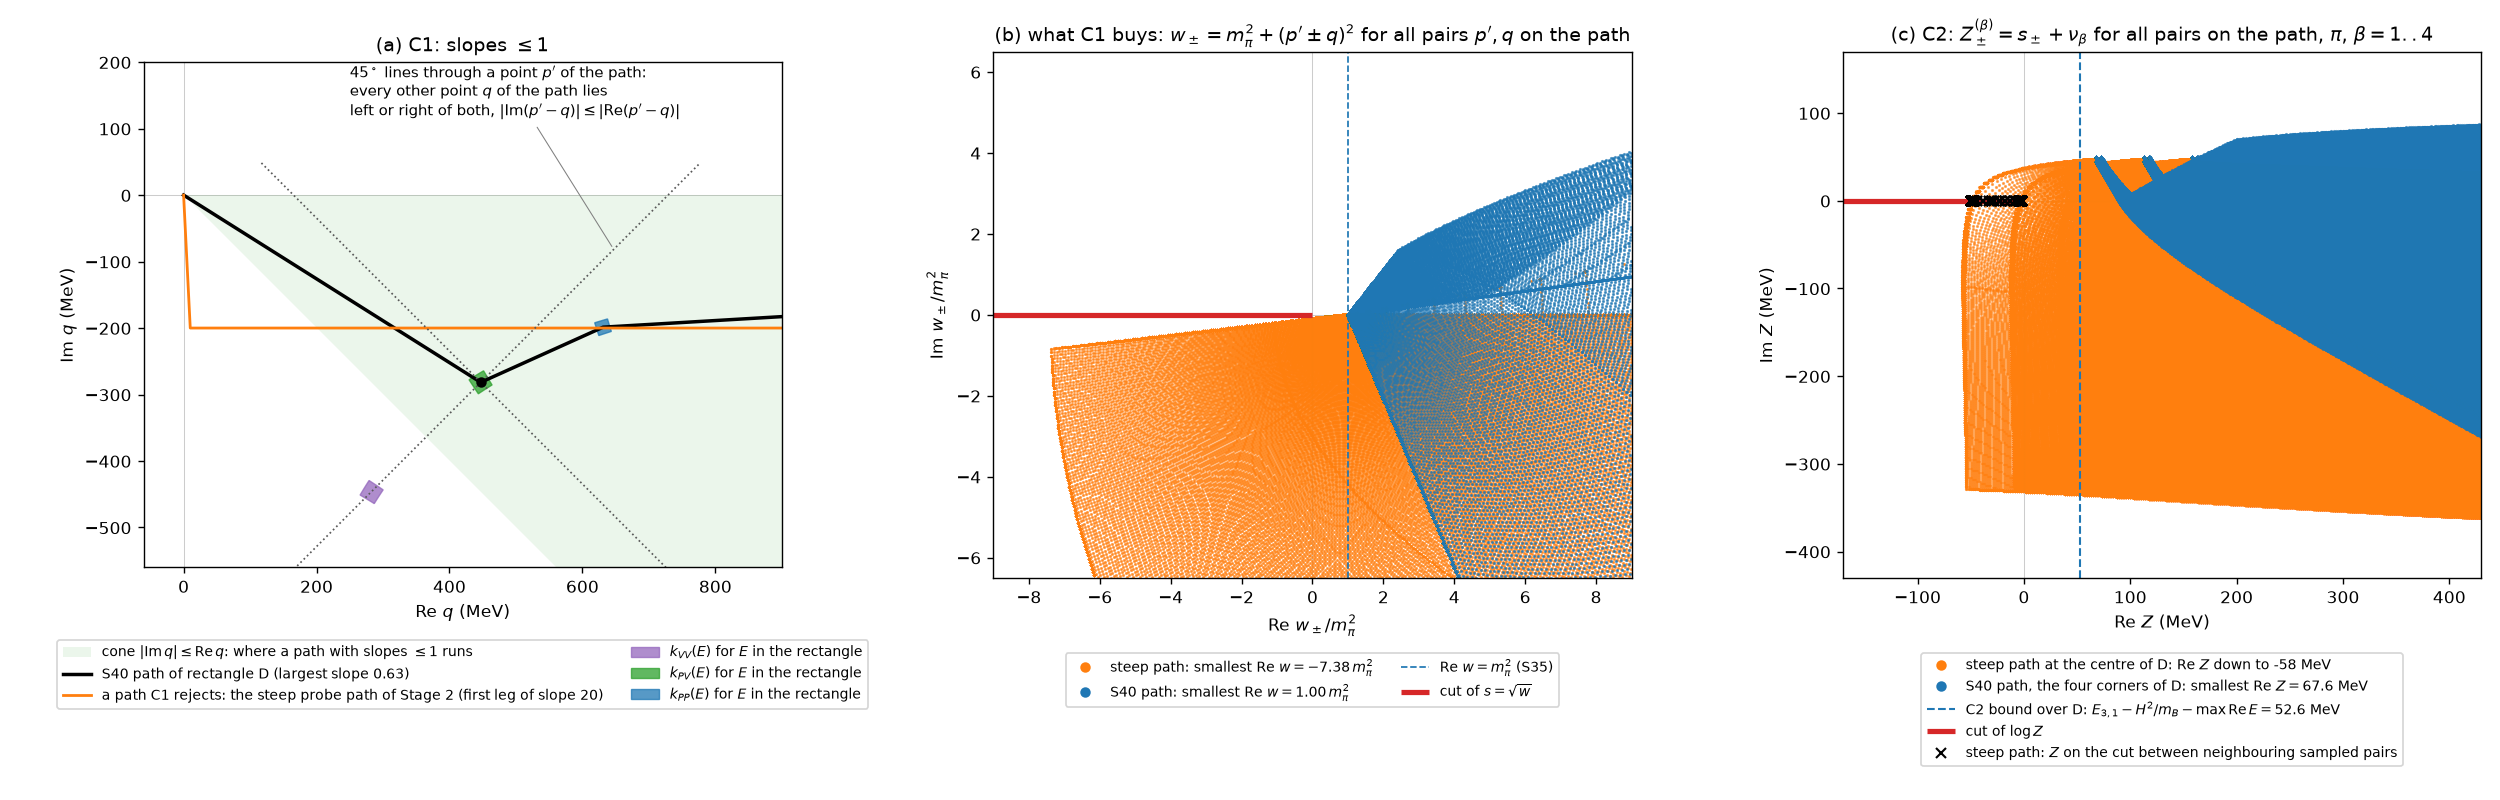
\includegraphics[width=\textwidth]{cert_path_pairs.png}
\caption{(C1) and (C2), pairs with both momenta on the path. (a) The path of a certified rectangle inside the cone $|\operatorname{Im}q|\le\operatorname{Re}q$, and the steep probe path of Stage~2. (b) $w_\pm$ for all sampled pairs, in units of $m_\pi^2$. (c) $Z^{(\beta)}_\pm$ for all sampled pairs, pion exchange, with the certified bound of (C2); crosses mark where $Z$ meets the cut on the steep path.}
\label{fig:certpairs}
\end{figure}

\begin{figure}[ht]
\centering
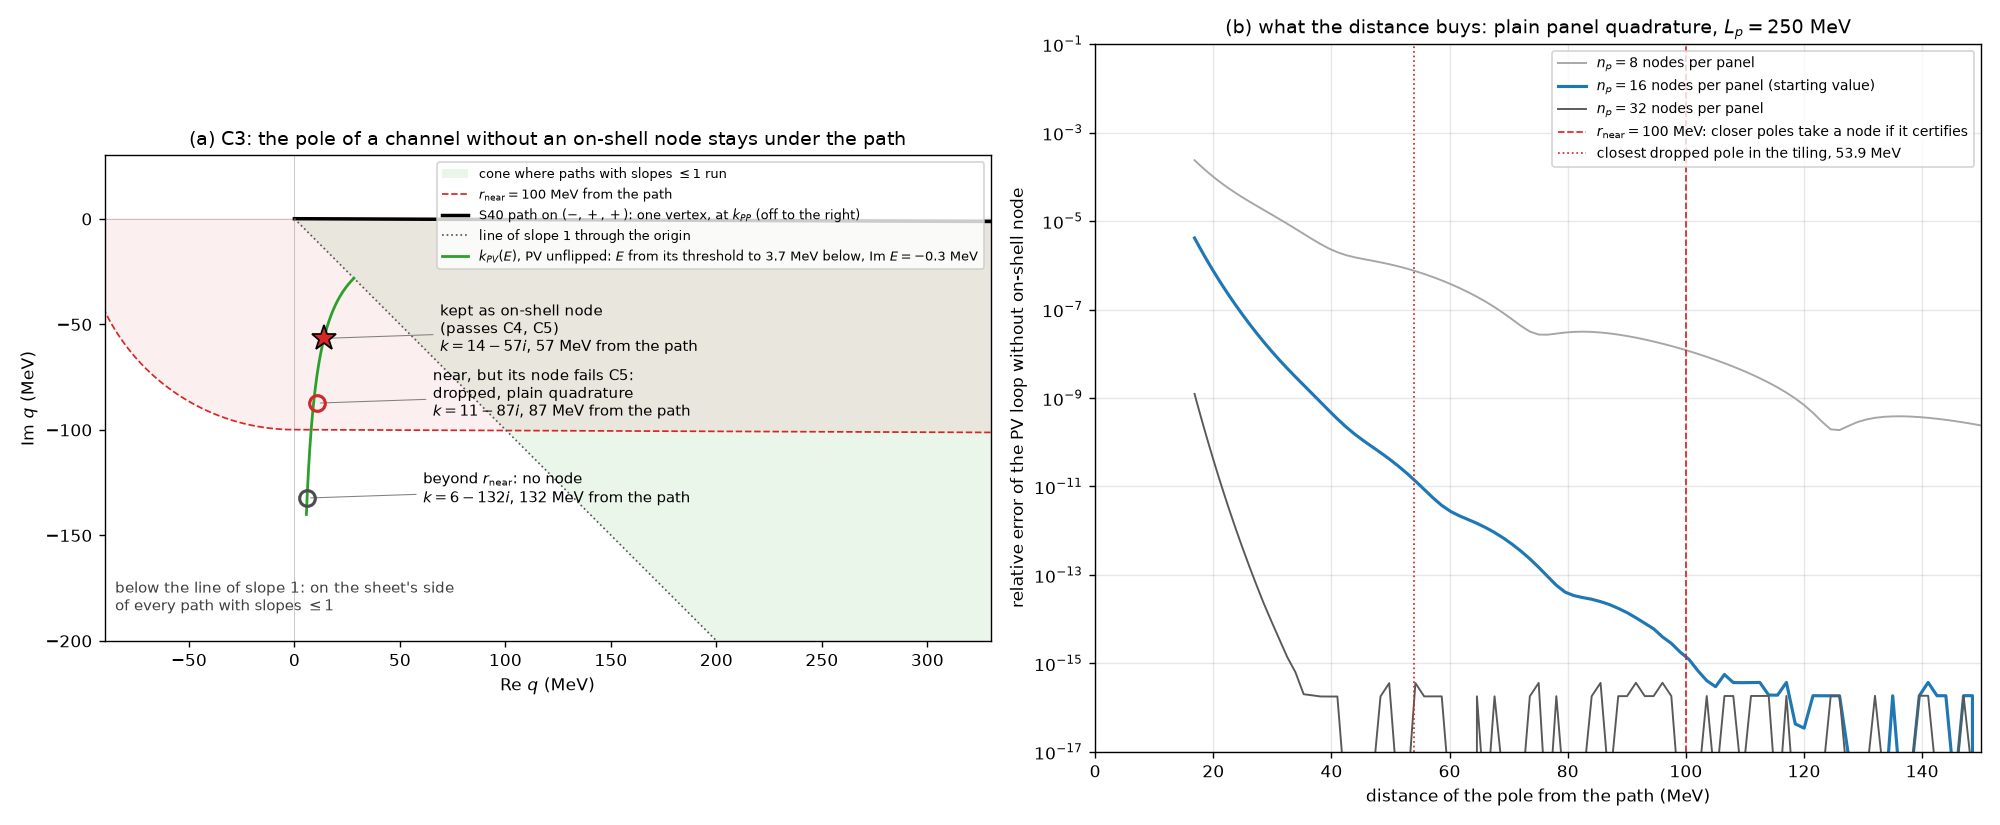
\includegraphics[width=\textwidth]{cert_poles.png}
\caption{(C3), a channel without an on-shell node. (a) The pole of $PV$, unflipped and just below its threshold, under the path on $(-,+,+)$: kept as an on-shell node, dropped, and beyond $r_{\rm near}$. (b) The relative error of that channel's loop by the plain panel quadrature against the distance of the pole from the path.}
\label{fig:certpoles}
\end{figure}

\begin{figure}[ht]
\centering
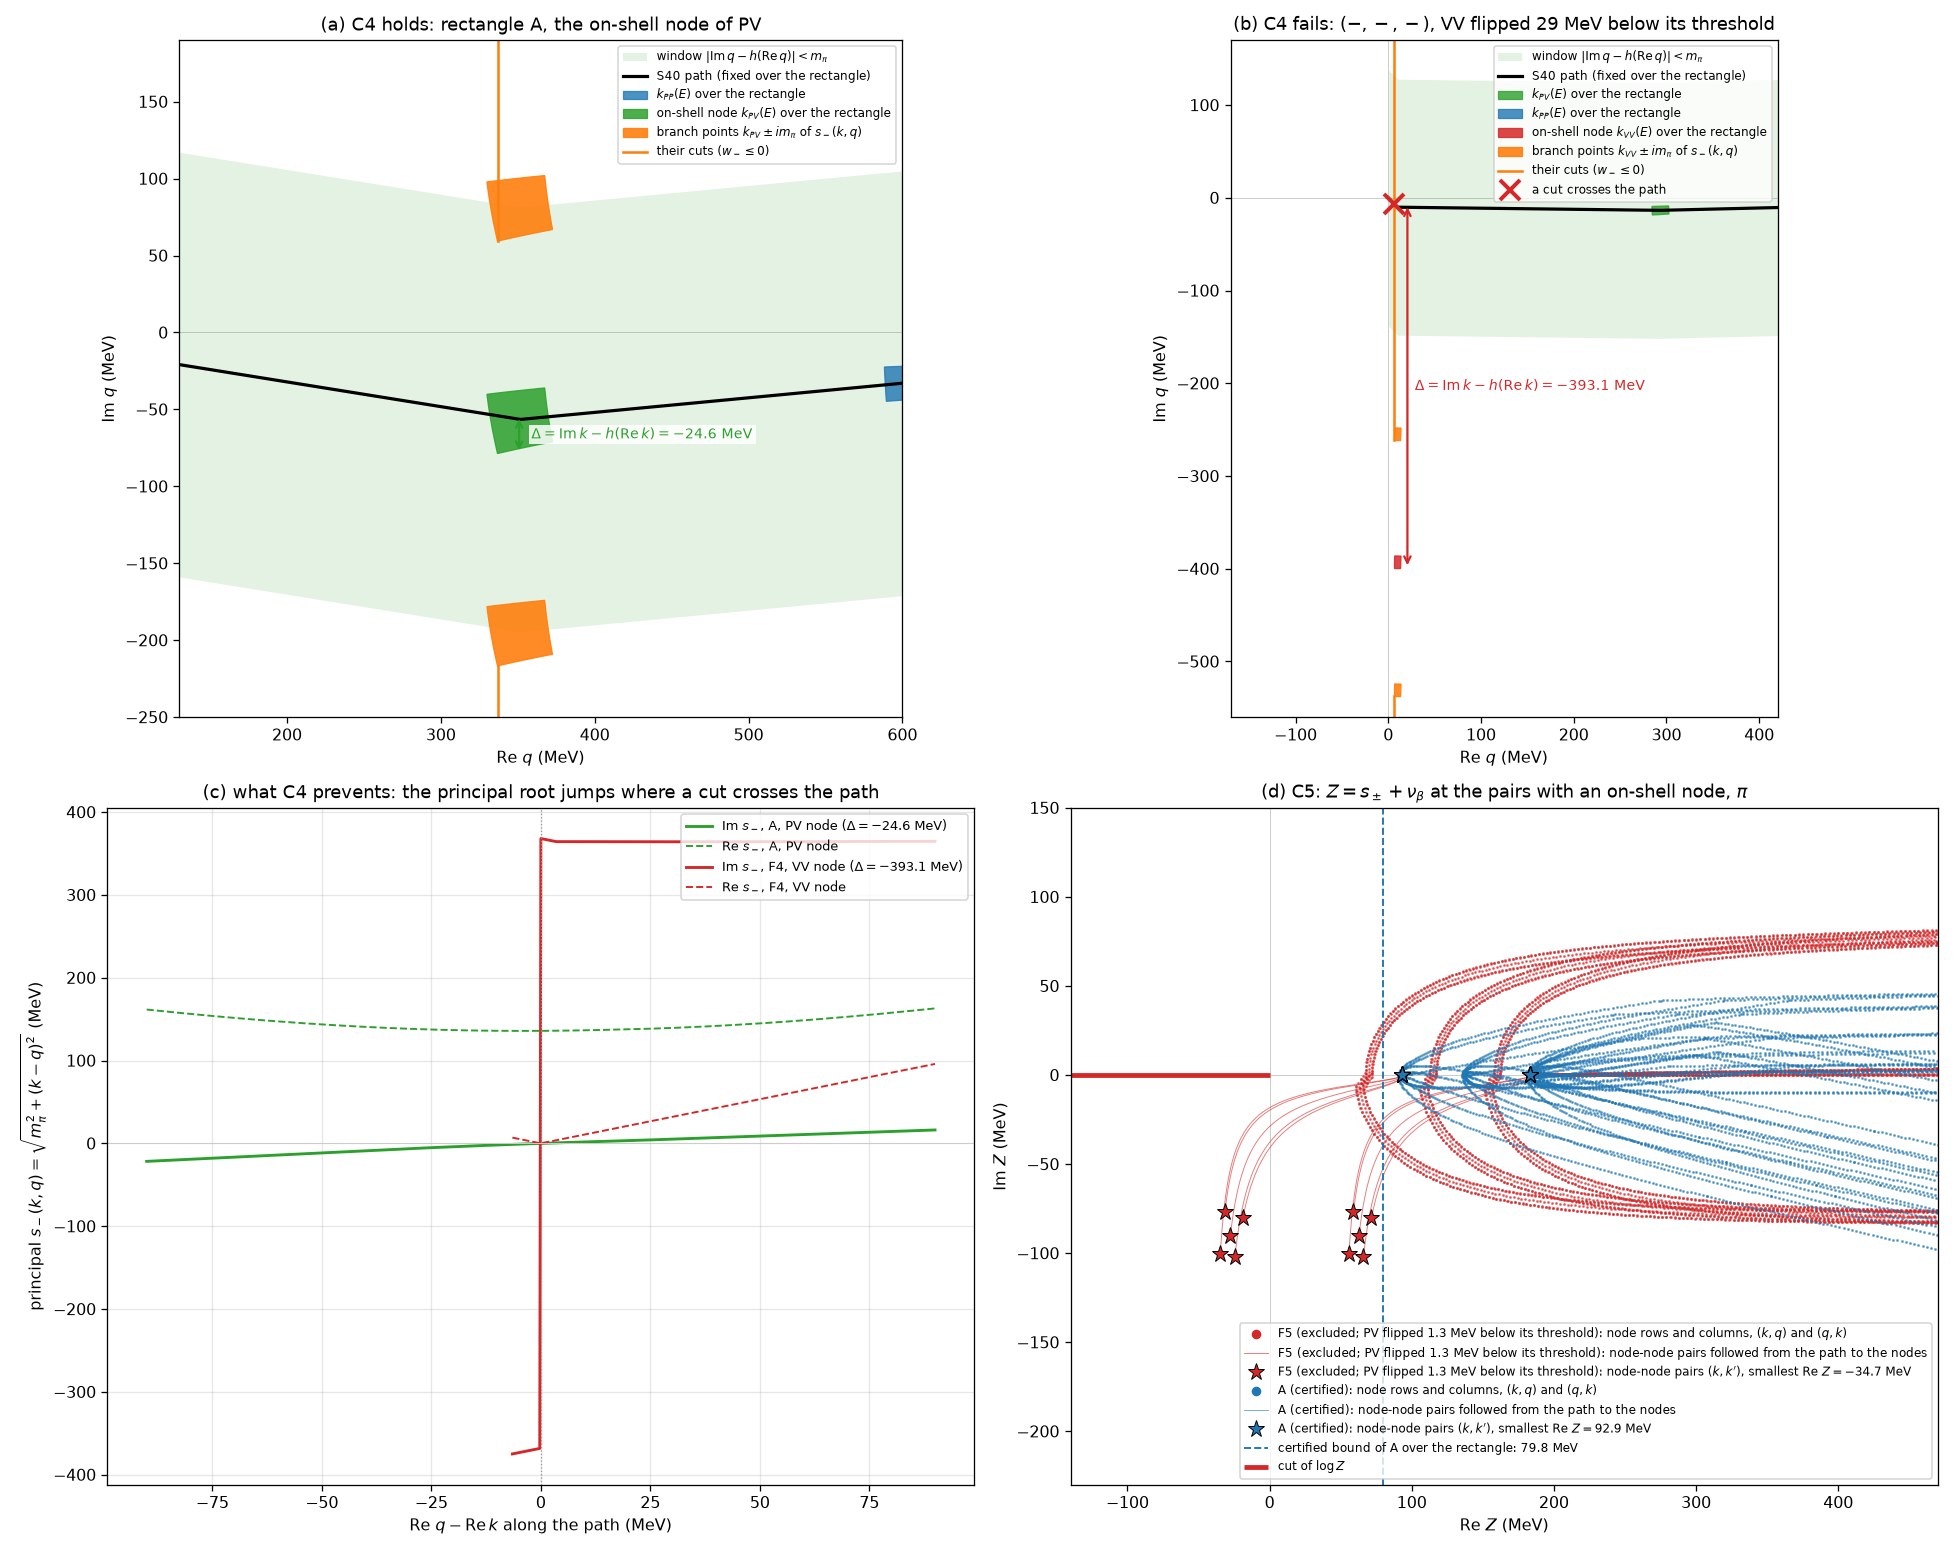
\includegraphics[width=\textwidth]{cert_nodes.png}
\caption{(C4) and (C5), pairs with an on-shell node. (a), (b) The window $|\operatorname{Im}q-h(\operatorname{Re}q)|<m_\pi$ around the path, the node momenta over the rectangle and the branch points $k\pm im_\pi$ of $s_-(k,q)$ with their cuts, where (C4) holds and where it fails. (c) The principal $s_-(k,q)$ along the path next to $\operatorname{Re}q=\operatorname{Re}k$. (d) $Z$ at the pairs with an on-shell node, on a certified rectangle and on one that (C5) excludes.}
\label{fig:certnodes}
\end{figure}

\begin{figure}[ht]
\centering
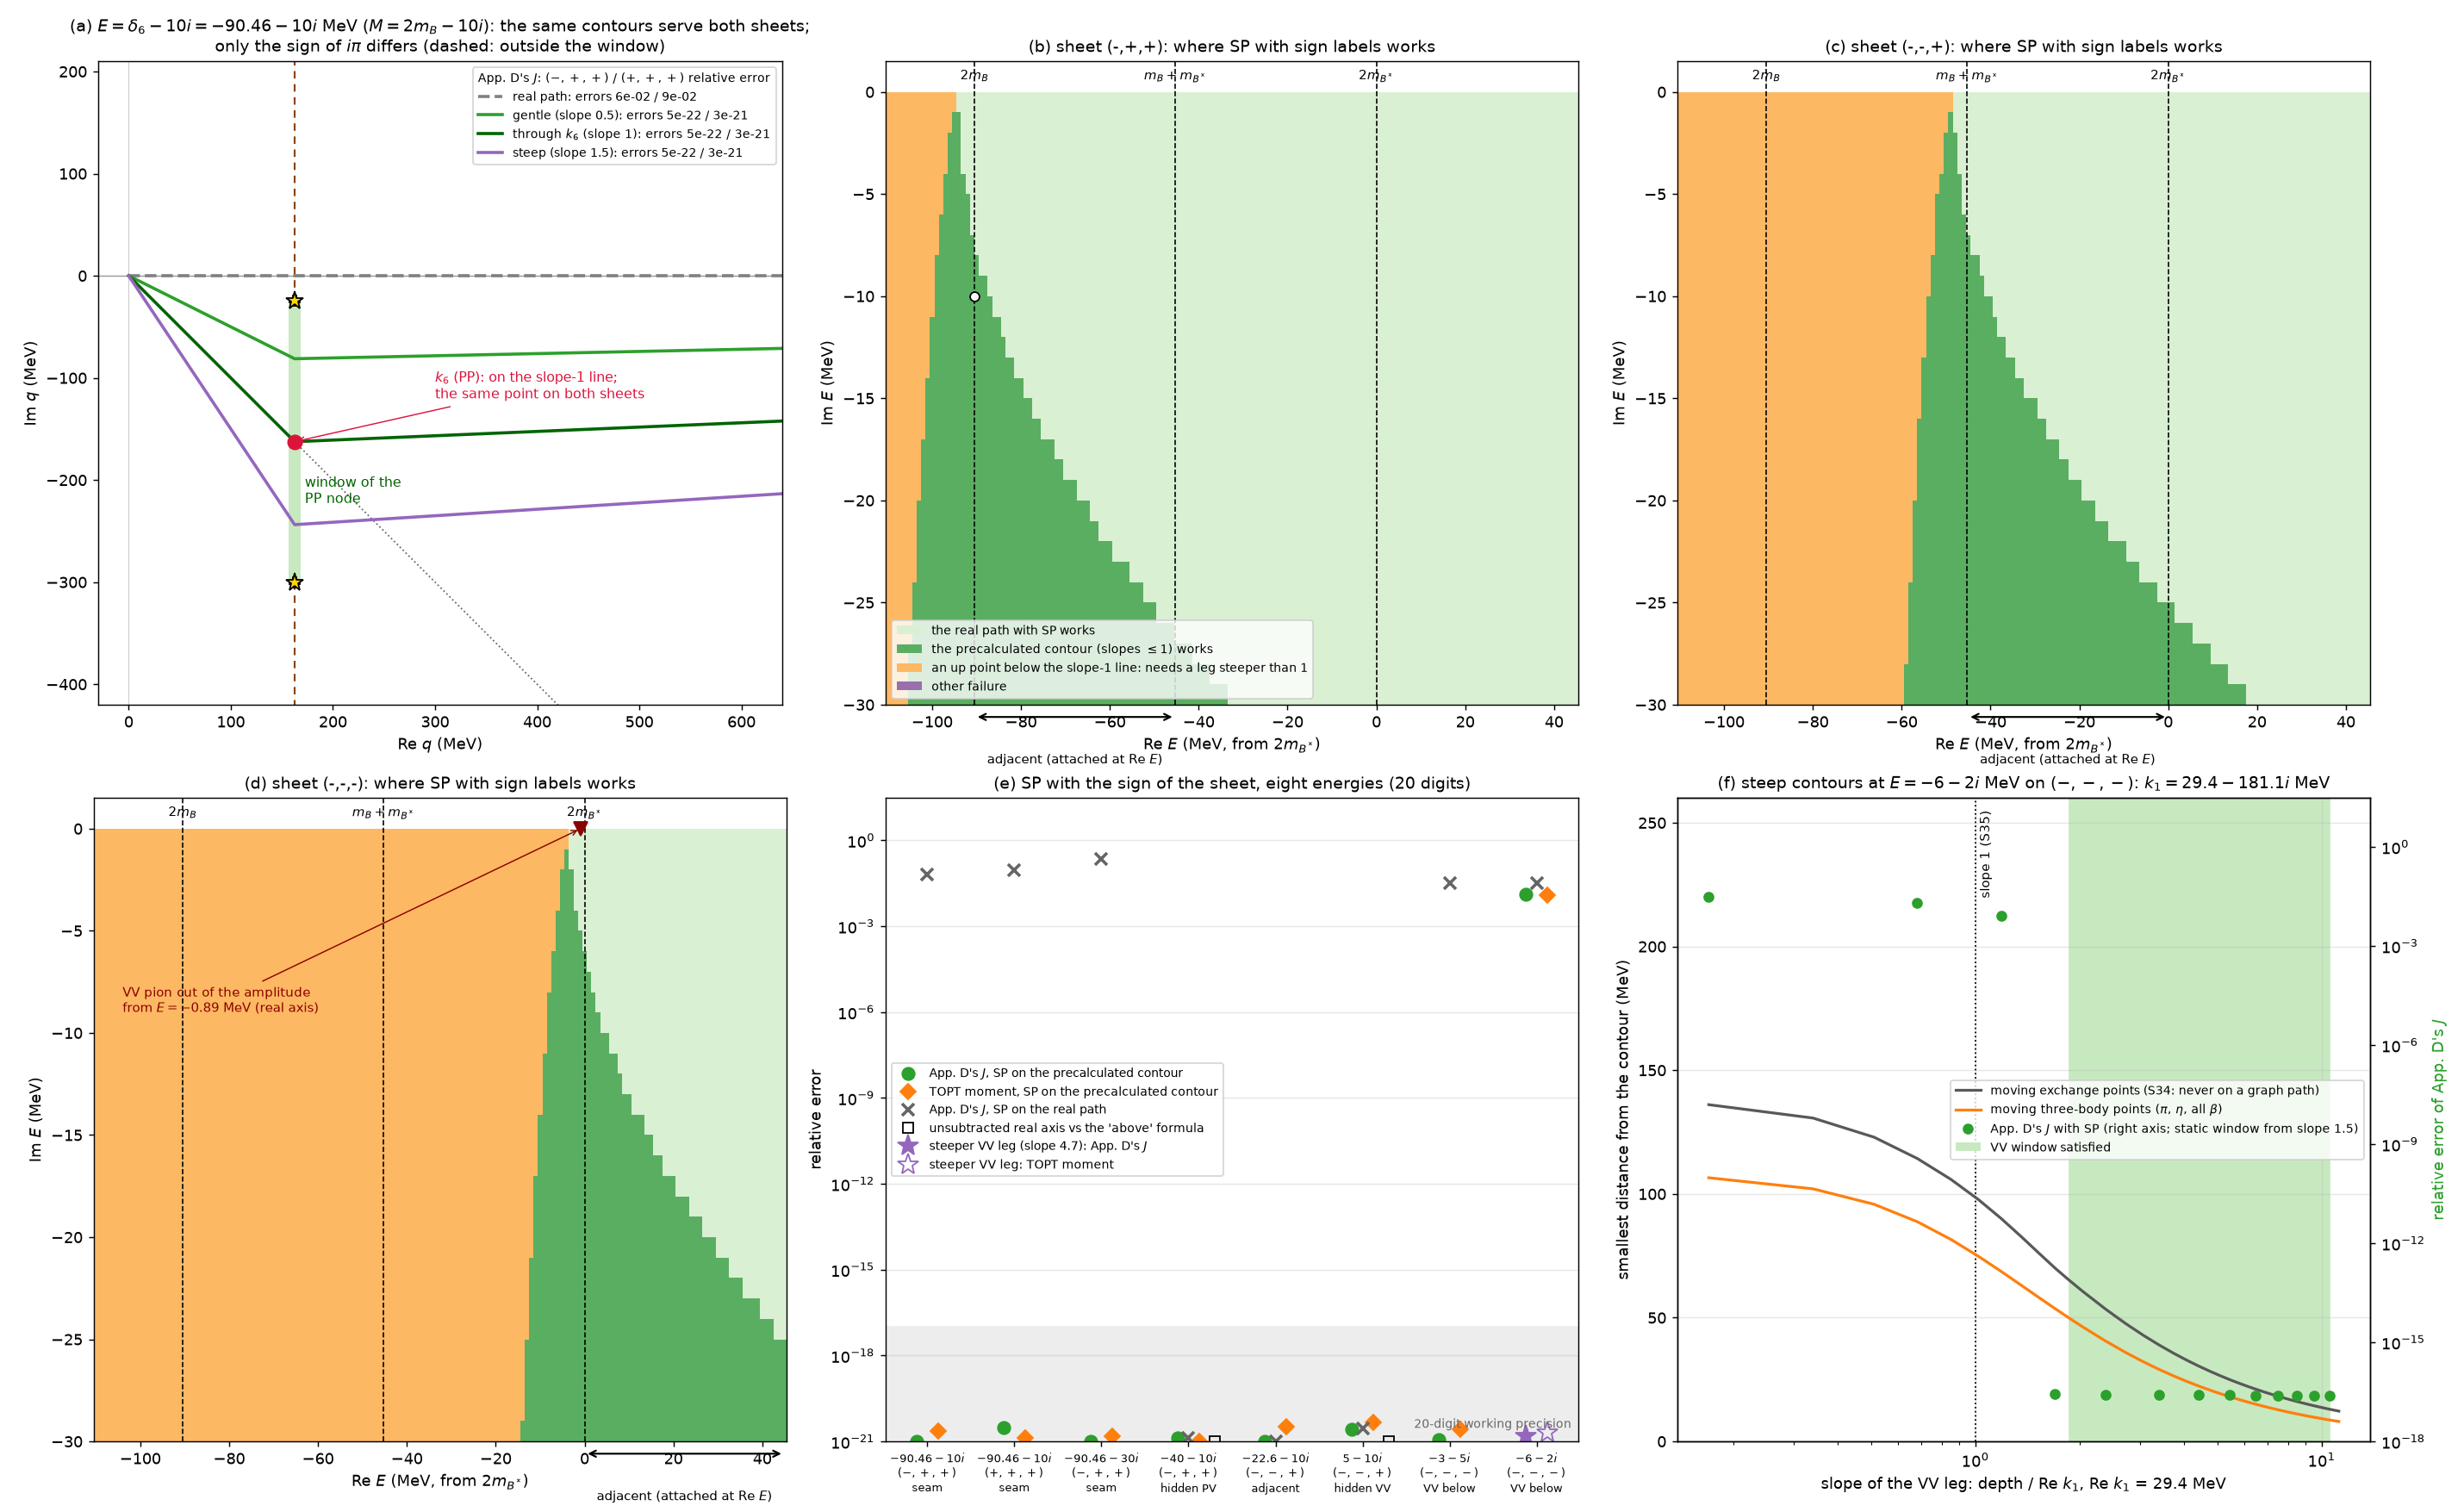
\includegraphics[width=\textwidth]{sp_sheets.png}
\caption{Sheet as a sign. (a) $E=\delta_6-10i$: the same contours serve $(-,+,+)$ and $(+,+,+)$; the real path fails, since $k_6+im_\pi$ lies below it. (b)--(d) Where the real path with Sokhotski--Plemelj suffices (light), where the precalculated path with slopes at most $1$ is valid (green), and where a steeper leg is needed (orange). (e) Eight energies at $20$ digits. (f) Steep legs at $E=-6-2i$ on $(-,-,-)$.}
\label{fig:sheets}
\end{figure}

\begin{figure}[ht]
\centering
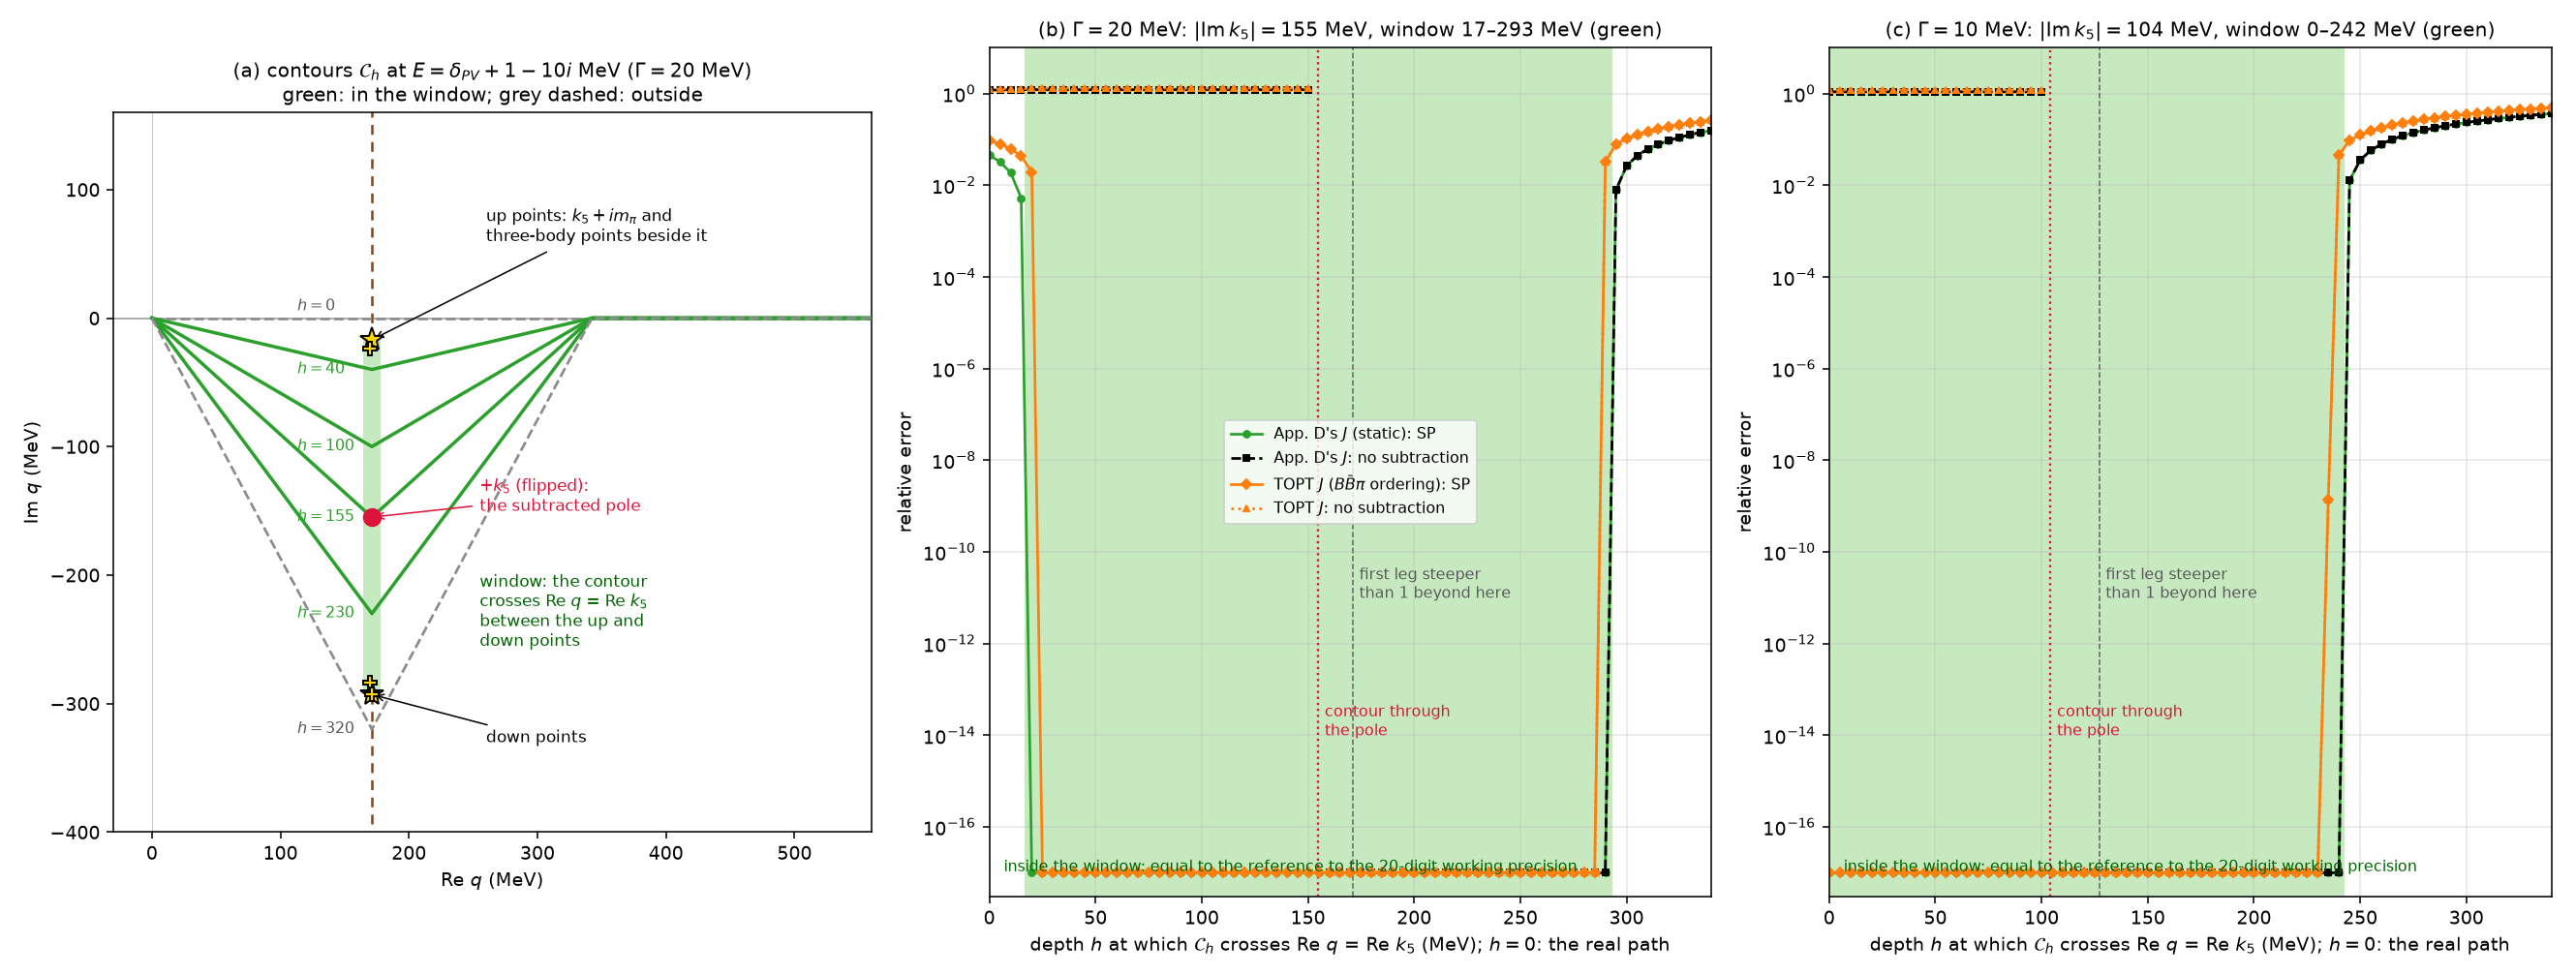
\includegraphics[width=\textwidth]{sp_window.png}
\caption{Sokhotski--Plemelj on the family $0\to\operatorname{Re}k_5-ih\to2\operatorname{Re}k_5\to$ real axis, $1$~MeV above the $PV$ threshold: exact for every depth $h$ inside the window, above or below the pole.}
\label{fig:window}
\end{figure}

\section{What changed in note 07}
\begin{itemize}
\item S40 is the rule of Sec.~\ref{sec:sign}: paths per rectangle, the panel quadrature R4, on-shell nodes with the sheet's sign, and the certificate (C1)--(C5); the remark after the path table (the margin $d_k$ limiting near thresholds) is replaced. The margin path of \texttt{graph\_path} stays as the second path of the Stage~6 path-independence check.
\item S9: an on-shell node adds one point per channel with the entry $W_\alpha/2\pi^2$; the sheet for this channel is fixed by the sign of its node term, not by which side the path passes.
\item S23 (P) and Decisions, Admissibility: a channel with an on-shell node may cross the path; (C4) and (C5) take the place of (P) for it.
\item S26: a pole with an on-shell node does not limit the convergence rate.
\item S32: with a node the path may pass $k_F$ on either side, with the window $|\Delta_F|<m_\pi$ and (C5).
\item S38 (V3): for Stage~7, the rectangle certificate of S40.
\item S41: each counting rectangle has its own certified path and node set and may straddle a threshold line.
\item Code: \texttt{sp\_path}, \texttt{panel\_rule}, \texttt{onshell\_nodes}, \texttt{certify\_rectangle} and \texttt{tile\_rectangles} in \file{code/Xb2Continuation}; the extra node rows and columns enter the Stage~6 solver.
\end{itemize}

\section{Choices}
\begin{enumerate}
\item Adopted (the user, 2026-11-13): the sheet-as-a-sign form of Sec.~\ref{sec:sign} as S40, with one certified path per rectangle and no required pole--vertex coincidence.
\item The starting quadrature, $L_p=250$~MeV and $n_p=16$, to be fixed by the Stage~6 node-doubling run against the targets ($0.1$~MeV for poles, $10^{-6}$ for on-shell $T$).
\item S35 without the $H^2$ term: needed only for the $(-,-,-)$ widening; adopt now or with it.
\item The grading towards $q=0$ next to $E_{3,1}$: decide with that widening.
\item A toy test before Stage~6 (\file{toy/}, to be agreed): on a three-channel static-Yukawa toy with the actual thresholds, does $D_{\mathcal C}$ on $\mathcal C(E)$ with R2 agree with $D_{\mathcal C}$ on the S40 path with graded nodes to $10^{-8}$ at probe energies of the first three rows, including $0.05$~MeV above each threshold and below $\delta_1$, and converge with $n_p\le24$? If yes, Stage~6 starts with the rule; if not, the reason is found first.
\end{enumerate}

\bibliography{../../refs}
\end{document}
